% =====================================================================
%  Trabalho de Graduação (TG) — FATEC Indaiatuba / ADS
%  Hierarquia de normas: Manual de Normas FATEC-ID (2021) > ABNT.
%  Compilar com: make   (pdflatex + bibtex + pdflatex x2)
% =====================================================================
\documentclass[
  12pt,
  oneside,
  a4paper,
  sumario=tradicional,
  brazil
]{abntex2}

% ----------------------------- Pacotes -------------------------------
\usepackage[T1]{fontenc}
\usepackage[utf8]{inputenc}
\usepackage{mathptmx}            % Times New Roman (texto e matemática)
\usepackage[brazil]{babel}
\usepackage{graphicx}
\usepackage{array}
\usepackage{booktabs}
\usepackage{multirow}
\usepackage{longtable}
\usepackage{amsmath,amssymb}
\usepackage{xcolor}
\usepackage{listings}
\usepackage{microtype}
\usepackage[alf]{abntex2cite}    % citações ABNT autor-data (estilo alf)

\graphicspath{{figuras/}}

% ----------------------- Ajustes de formatação -----------------------
% Manual FATEC: recuo de primeira linha 1,25 cm; espaçamento 1,5;
% sem afastamento entre parágrafos; margens 3/2/3/2 (padrão abnTeX2).
\setlength{\parindent}{1.25cm}
\setlength{\parskip}{0pt}

% --- Estilo de títulos (Manual FATEC 1.3 e 4.2.2) --------------------
% Capítulo: 14 pt, negrito, só inicial maiúscula, alinhado à esquerda.
% Subtítulos (seção/subseção): 12 pt, negrito, alinhados à esquerda.
\renewcommand{\chaptitlefont}{\normalfont\bfseries\fontsize{14}{18}\selectfont}
\renewcommand{\chapnumfont}{\chaptitlefont}
% O abnTeX2 redefine \chaptitlefont no \AtBeginDocument; reaplicamos DEPOIS
% para garantir que o tamanho dos títulos seja realmente respeitado.
% Manual FATEC 1.3: títulos = 14 pt. (Para aproximar do PDF original, use 12.)
\AtBeginDocument{%
  \renewcommand{\chaptitlefont}{\normalfont\bfseries\fontsize{14}{18}\selectfont}%
  \renewcommand{\chapnumfont}{\chaptitlefont}%
}

% Rótulo de divisão centralizado (INTRODUÇÃO, CAPÍTULO I, ...).
\newif\ifhasdiv
\newcommand{\divlabel}{}
\newcommand{\setdiv}[1]{\hasdivtrue\renewcommand{\divlabel}{#1}}
\newif\ifchapnumbered

% Estilo de capítulo:
%  - capítulo numerado  -> "N Título" à esquerda, só inicial maiúscula;
%  - capítulo sem número (pré-textual/REFERÊNCIAS) -> centralizado, CAIXA-ALTA;
%  - rótulo de divisão (INTRODUÇÃO/CAPÍTULO) centralizado acima do título.
\makechapterstyle{fatec}{%
  \setlength{\beforechapskip}{0pt}
  \setlength{\afterchapskip}{\onelineskip}
  \setlength{\midchapskip}{0pt}
  \renewcommand{\chapterheadstart}{%
    \chapnumberedfalse
    \ifhasdiv
      \phantomsection
      \addcontentsline{toc}{chapter}{\divlabel}%
      {\centering\chaptitlefont\divlabel\par}%
      \vskip\onelineskip
      \hasdivfalse
    \fi
  }%
  \renewcommand{\printchaptername}{}%
  \renewcommand{\chapternamenum}{}%
  \renewcommand{\printchapternum}{\chapnumberedtrue\chaptitlefont\thechapter\hspace{0.5em}}%
  \renewcommand{\afterchapternum}{}%
  \renewcommand{\printchaptertitle}[1]{%
    \ifchapnumbered
      \chaptitlefont ##1%
    \else
      {\centering\chaptitlefont\MakeTextUppercase{##1}\par}%
    \fi}%
  \renewcommand{\afterchaptertitle}{\par\nobreak\vskip\onelineskip}%
}
\chapterstyle{fatec}

% Paginação: apenas o número no canto superior direito, sem cabeçalho
% corrente nem filete (Manual FATEC 1.5).
\makepagestyle{numtopright}
\makeevenhead{numtopright}{\thepage}{}{}
\makeoddhead{numtopright}{}{}{\thepage}
\makeheadrule{numtopright}{0pt}{0pt}
\makeevenfoot{numtopright}{}{}{}
\makeoddfoot{numtopright}{}{}{}
\aliaspagestyle{chapter}{numtopright}

% Títulos pré-textuais (RESUMO, SUMÁRIO, LISTA DE..., REFERÊNCIAS):
% abnTeX2 usa, por padrão, sans-serif \Huge — o Manual FATEC pede Times 14.
\renewcommand{\ABNTEXchapterfont}{\normalfont\bfseries\fontsize{14}{18}\selectfont}
\renewcommand{\ABNTEXchapterfontsize}{\fontsize{14}{18}\selectfont}
\renewcommand{\resumoname}{RESUMO}
\renewcommand{\bibname}{REFERÊNCIAS}
\renewcommand{\apendicesname}{APÊNDICES}

% Seções e subseções: 12 pt negrito, à esquerda (sem caixa-alta).
\setsecheadstyle{\normalfont\bfseries\fontsize{12}{16}\selectfont\raggedright}
\setsubsecheadstyle{\normalfont\bfseries\fontsize{12}{16}\selectfont\raggedright}
\setsubsubsecheadstyle{\normalfont\bfseries\fontsize{12}{16}\selectfont\raggedright}

% --- Sumário: 2 níveis (capítulo e seção); 1.1.1 omitido; todas as
%     entradas à esquerda (sem identação progressiva) e em negrito;
%     pontilhado denso em todos os níveis (Manual 1.5 + legibilidade).
\makeatletter
\renewcommand{\l@subsection}[2]{}              % omite 1.1.1 do sumário
\renewcommand{\l@part}[2]{}                     % omite "APÊNDICES" do sumário
\renewcommand{\l@appendix}[2]{}                 % omite "APÊNDICE A" do sumário
\makeatother
\renewcommand{\cftdotsep}{1}                    % pontilhado populado
\renewcommand{\cftchapterdotsep}{\cftdotsep}    % pontilhado também nos capítulos
\renewcommand{\cftsectiondotsep}{\cftdotsep}
\renewcommand*{\cftchapterfont}{\normalfont\bfseries}        % títulos em negrito
\renewcommand*{\cftsectionfont}{\normalfont}                 % subseções sem negrito
\renewcommand*{\cftchapterpagefont}{\normalfont\bfseries}
\renewcommand*{\cftsectionpagefont}{\normalfont}
\cftsetindents{chapter}{0em}{1.4em}
\cftsetindents{section}{0em}{2.6em}
\setlength{\cftbeforepartskip}{0pt}            % apêndice omitido do sumário

% Garante nomes em caixa-alta no sumário (babel reescreve esses rótulos).
\addto\captionsbrazil{%
  \renewcommand{\bibname}{REFERÊNCIAS}%
  \renewcommand{\apendicesname}{APÊNDICES}%
  \renewcommand{\anexosname}{ANEXOS}%
  \renewcommand{\listfigurename}{LISTA DE FIGURAS}%
  \renewcommand{\listtablename}{LISTA DE TABELAS}%
}
\renewcommand{\listfigurename}{LISTA DE FIGURAS}
\renewcommand{\listtablename}{LISTA DE TABELAS}

% --- Legendas de ilustrações/tabelas (Manual FATEC 1.3 e seção 3) -----
% Tamanho 10, "Figura N" em negrito, travessão, legenda em cima e fonte
% logo abaixo da ilustração.
\renewcommand{\ABNTEXfontereduzida}{\fontsize{10}{12}\selectfont}
\captionnamefont{\fontsize{10}{12}\selectfont\bfseries}
\captiontitlefont{\fontsize{10}{12}\selectfont}
\captiondelim{\space--\space}
\captionstyle{\centering}
\setlength{\abovecaptionskip}{2pt}
\setlength{\belowcaptionskip}{2pt}
% A linha de fonte usa o comando nativo \fonte{...} do abnTeX2,
% que imprime "Fonte: ..." em tamanho reduzido.

% --- Estilo do código MQL5 (Apêndice A) ------------------------------
\definecolor{codegray}{gray}{0.4}
\definecolor{codegreen}{rgb}{0,0.5,0}
\definecolor{codeblue}{rgb}{0,0,0.6}
\lstdefinestyle{mql5}{
  language=C++,
  basicstyle=\ttfamily\fontsize{8}{9}\selectfont,
  keywordstyle=\color{codeblue}\bfseries,
  commentstyle=\color{codegreen},
  stringstyle=\color{codegray},
  numbers=left,
  numberstyle=\tiny\color{codegray},
  numbersep=8pt,
  breaklines=true,
  showstringspaces=false,
  tabsize=2,
  extendedchars=true,
  literate=%
    {á}{{\'a}}1 {é}{{\'e}}1 {í}{{\'i}}1 {ó}{{\'o}}1 {ú}{{\'u}}1
    {â}{{\^a}}1 {ê}{{\^e}}1 {ô}{{\^o}}1 {ã}{{\~a}}1 {õ}{{\~o}}1
    {ç}{{\c c}}1 {à}{{\`a}}1 {Á}{{\'A}}1 {É}{{\'E}}1 {Ç}{{\c C}}1
    {ô}{{\^o}}1 {Ã}{{\~A}}1 {Õ}{{\~O}}1 {â}{{\^a}}1,
  morekeywords={input,datetime,ulong,double,int,bool,string,void,
    OnInit,OnTick,OnDeinit,CTrade,MqlTick,ENUM_MA_METHOD,
    ENUM_APPLIED_PRICE,ENUM_POSITION_TYPE,iMA,CopyBuffer,
    SymbolInfoTick,SymbolInfoInteger,SymbolInfoDouble,NormalizeDouble,
    PositionsTotal,PositionGetTicket,PositionSelectByTicket,
    PositionGetString,PositionGetInteger,SeriesInfoInteger}
}

% Metadados PDF
\usepackage{hyperref}
\hypersetup{
  pdftitle={Previsão e Análise de Tendências no Mercado de Ativos},
  pdfauthor={Bruno Rocha Pereira e Giovanni Silva Loose},
  colorlinks=false, pdfborder={0 0 0}
}

% =====================================================================
\begin{document}

% ------------------------- Elementos pré-textuais --------------------
\pretextual

% Capa — Manual FATEC 4.1.2
% Instituição e autor no alto (centralizado, MAIÚSCULAS, 14, espaço duplo);
% título no centro (negrito, minúsculas, 16); local/ano na base (14).
\begin{capa}
\thispagestyle{empty}
\center

{\fontsize{14}{22}\selectfont
\MakeUppercase{Centro Estadual de Educação Tecnológica Paula Souza}\\
\MakeUppercase{Faculdade de Tecnologia de Indaiatuba}\\
\MakeUppercase{Dr. Archimedes Lamoglia}\\
\MakeUppercase{Curso de Tecnologia}\\
\MakeUppercase{em Análise e Desenvolvimento de Sistemas}\par}

\vspace{0.12\textheight}

{\fontsize{14}{18}\selectfont
\MakeUppercase{Bruno Rocha Pereira e Giovanni Silva Loose}\par}

\vfill

% Obs: o Manual FATEC 4.1.2 especifica 16 pt; aqui usa-se 14 pt para
% reproduzir o espaçamento/tamanho original.
{\bfseries\fontsize{14}{17}\selectfont
Previsão e Análise de Tendências no Mercado de Ativos:\\
Desenvolvimento de Ferramenta Algorítmica com Modelos\\
Estatísticos no MetaTrader 5\par}

\vfill

{\fontsize{14}{18}\selectfont
Indaiatuba\\
2025\par}

\end{capa}

% Folha de rosto — Manual FATEC 4.1.4
% Nota de apresentação justificada (Times 12),
% recuada a 7 cm da margem esquerda.
\begin{folhaderosto}
\thispagestyle{empty}
\center

{\fontsize{14}{22}\selectfont
\MakeUppercase{Centro Estadual de Educação Tecnológica Paula Souza}\\
\MakeUppercase{Faculdade de Tecnologia de Indaiatuba}\\
\MakeUppercase{Dr. Archimedes Lamoglia}\\
\MakeUppercase{Curso de Tecnologia}\\
\MakeUppercase{em Análise e Desenvolvimento de Sistemas}\par}

\vspace{0.12\textheight}

{\fontsize{14}{18}\selectfont
\MakeUppercase{Bruno Rocha Pereira e Giovanni Silva Loose}\par}

\vfill

{\bfseries\fontsize{14}{17}\selectfont
Previsão e Análise de Tendências no Mercado de Ativos:\\
Desenvolvimento de Ferramenta Algorítmica com Modelos\\
Estatísticos no MetaTrader 5\par}

\vspace{\onelineskip}

\hfill\begin{minipage}{\dimexpr\textwidth-7cm\relax}
\SingleSpacing\fontsize{12}{14}\selectfont
Projeto de trabalho de graduação apresentado por Bruno Rocha Pereira e
Giovanni Silva Loose como pré-requisito para a conclusão do Curso Superior
de Tecnologia em Análise e Desenvolvimento de Sistemas, da Faculdade de
Tecnologia de Indaiatuba, elaborado sob a orientação do Prof. MsC. Michel
Moron Munhoz.
\end{minipage}

\vfill

{\fontsize{14}{18}\selectfont
Indaiatuba\\
2025\par}

\end{folhaderosto}

% \input{conteudo/folha-aprovacao}  % obrigatória só na versão final

% Resumo — Manual FATEC 4.1.10 (parágrafo único, espaçamento simples,
% palavras-chave separadas e finalizadas por ponto).
\begin{resumo}
O cenário econômico brasileiro recente, caracterizado por instabilidade
macroeconômica, inflação elevada e consequente aumento da taxa Selic, impõe
desafios significativos aos investidores. A volatilidade do mercado financeiro,
intensificada por fatores internos e externos, dificulta a tomada de decisões de
investimento, especialmente em ativos como ações. Diante desse contexto e da
crescente digitalização do setor financeiro, o trading algorítmico apresenta-se como
uma alternativa promissora. Este trabalho apresenta o desenvolvimento de um algoritmo de
negociação, escrito na linguagem MQL5 para a plataforma MetaTrader 5, para
análise de padrões de tendência e volatilidade no mercado de ações brasileiro,
tomando como base o ativo PETR4. O algoritmo integra análises técnicas
estatísticas, combinando o uso de Médias Móveis para identificação de tendências
e os modelos ARIMA para previsão de séries temporais de preços e GARCH para
modelagem da volatilidade condicional dos resíduos do ARIMA. A premissa central
deste trabalho é que essa abordagem integrada permite a geração de sinais de
negociação com maior eficácia (potencial de acerto e adequação ao risco) em
comparação com o uso isolado ou incompleto dessas técnicas. O estudo explorou
modelos com dados atualizados, fornecendo análises que possam embasar estratégias de
investimento adaptadas ao cenário de juros altos e investigando a robustez da
combinação de modelos ARIMA e GARCH frente às flutuações do mercado, contribuindo para o
conhecimento na área e oferecendo uma alternativa prática para investidores.

\vspace{\onelineskip}
\noindent\textbf{Palavras-chave:} Trading Algorítmico. Modelos Estatísticos. ARIMA.
GARCH. Mercado de Ações. Bolsa de Valores. Volatilidade. MetaTrader 5.
\end{resumo}

% Abstract — Manual FATEC 4.1.11 (versão do resumo em língua estrangeira).
% No original, o texto do abstract é apresentado em itálico.
\begin{resumo}[ABSTRACT]
\begin{otherlanguage}{english}
\itshape
The recent Brazilian economic scenario, characterized by macroeconomic
instability, high inflation, and a consequent increase in the Selic interest rate,
poses significant challenges for investors. Financial market volatility,
intensified by internal and external factors, hinders investment decision-making,
especially in assets such as stocks. Given this context and the increasing
digitalization of the financial sector, algorithmic trading presents itself as a promising
alternative. This paper presents the development of a computational tool, using
the MQL5 language on the MetaTrader 5 platform, for analyzing trend and volatility
patterns in the Brazilian stock market, focusing on the PETR4 asset. The tool integrates
statistical technical analyses, combining the use of Moving Averages for
trend identification with the ARIMA model for forecasting price time series and the GARCH
model for modeling the conditional volatility of ARIMA residuals. The central
premise of this work is that this integrated approach allows the generation of trading
signals with greater effectiveness (potential accuracy and risk suitability)
compared to the isolated or incomplete use of these techniques. The study explored
models with updated data, providing analyses that can support investment
strategies adapted to the high-interest-rate scenario, and investigated the
robustness of the combined ARIMA and GARCH models against market fluctuations, contributing to
knowledge in the field and offering a practical alternative for investors.

\vspace{\onelineskip}
\noindent\textbf{Keywords:} Algorithmic Trading. Statistical Models. ARIMA. GARCH.
Stock Market. Volatility. MetaTrader 5.
\end{otherlanguage}
\end{resumo}


% Listas (mín. 5 itens cada -> listas próprias, Manual 4.1.12)
\pdfbookmark[0]{Lista de figuras}{lof}
\listoffigures*
\cleardoublepage

\pdfbookmark[0]{Lista de tabelas}{lot}
\listoftables*
\cleardoublepage

% Lista de siglas — Manual FATEC 4.1.14 (ordem alfabética).
\pdfbookmark[0]{Lista de siglas}{losiglas}
\chapter*{Lista de siglas}
\begingroup
\SingleSpacing
\renewcommand{\arraystretch}{1.6}
\noindent\begin{tabular}{@{}l@{\hspace{1em}}l@{}}
\textbf{ADF}    & Augmented Dickey-Fuller \\
\textbf{AIC}    & Akaike Information Criterion \\
\textbf{API}    & Application Programming Interface \\
\textbf{ARIMA}  & AutoRegressive Integrated Moving Average \\
\textbf{Copom}  & Comitê de Política Monetária \\
\textbf{EA}     & Expert Advisor \\
\textbf{GARCH}  & Generalized Autoregressive Conditional Heteroskedasticity \\
\textbf{IFR}    & Índice de Força Relativa \\
\textbf{MAE}    & Mean Absolute Error \\
\textbf{MACD}   & Moving Average Convergence Divergence \\
\textbf{MM}     & Média Móvel \\
\textbf{MME}    & Média Móvel Exponencial \\
\textbf{MMS}    & Média Móvel Simples \\
\textbf{MQL5}   & MetaQuotes Language 5 \\
\textbf{MT5}    & MetaTrader 5 \\
\textbf{PETR4}  & Código de negociação das ações preferenciais da Petrobras \\
\textbf{PIB}    & Produto Interno Bruto \\
\textbf{RMSE}   & Root Mean Square Error \\
\textbf{RSI}    & Relative Strength Index \\
\textbf{SELIC}  & Sistema Especial de Liquidação e de Custódia \\
\textbf{SL}     & Stop Loss \\
\textbf{TG}     & Trabalho de Graduação \\
\textbf{TP}     & Take Profit \\
\end{tabular}
\endgroup
\cleardoublepage


% Sumário (Manual 4.1.14: pré-textuais não constam)
\pdfbookmark[0]{Sumário}{toc}
\tableofcontents*
\cleardoublepage

% ------------------------- Elementos textuais ------------------------
\textual
\pagestyle{numtopright}

% =====================================================================
%  INTRODUÇÃO / 1 Contextualização
% =====================================================================
\setdiv{INTRODUÇÃO}
\chapter{Contextualização}

Nos últimos anos, a economia brasileira tem enfrentado um cenário desafiador,
marcado por instabilidade macroeconômica e oscilações no mercado financeiro. Para
tentar controlar a inflação pressionada pela alta do dólar e pelos desafios nas
contas públicas, o Banco Central tem buscado contê-la por meio do aumento da taxa
Selic, que alcançou 14,25\% ao ano e pode ultrapassar 15\%.

Definida periodicamente pelo Comitê de Política Monetária (Copom), essa taxa
reflete as condições macroeconômicas do país e as expectativas para a inflação em
2025, segundo previsões de instituições financeiras como Citi, Itaú e XP
\cite{ayres2025}.

Esse aumento da Selic reflete preocupações com a inflação, que vem subindo não só
pelo custo maior de produtos importados, consequência direta da desvalorização do
Real, mas também por fatores internos, como o consumo elevado e a falta de
confiança na estabilidade fiscal do país. Essa instabilidade do mercado financeiro
está diretamente relacionada à política monetária adotada pelo Banco Central, com
destaque para a taxa Selic. Como principal instrumento para o controle da inflação
e a regulação da atividade econômica, a Selic influencia diretamente outras taxas
de juros, como as de empréstimos, financiamentos e aplicações financeiras
\cite{bcbSelic}. Mudanças significativas na Selic podem alterar a dinâmica do
mercado financeiro, impactando tanto o custo do crédito quanto o retorno dos
investimentos.

\begin{table}[htb]
\centering
\caption{Variações da SELIC anual, Meta e Real (2020-2025*)}
\label{tab:selic}
\fontsize{10}{12}\selectfont
\begin{tabular}{ccc}
\toprule
\textbf{Ano} & \textbf{SELIC Meta (\%)} & \textbf{SELIC Real (\%)} \\
\midrule
2025 & 14,25* & -- \\
2024 & 12,25 & 12,15 \\
2023 & 11,75 & 11,65 \\
2022 & 13,75 & 13,65 \\
2021 & 9,25 & 9,15 \\
2020 & 2,00 & 1,90 \\
\bottomrule
\end{tabular}

\vspace{2pt}
{\fontsize{10}{12}\selectfont Fonte: Banco Central do Brasil (2025).}
\end{table}

Apesar do cenário desafiador, a economia brasileira continua crescendo, com um
avanço de 3,3\% em 2024 e previsão de 2,5\% para 2025 no PIB \cite{ayres2024}. No
entanto, esse crescimento acontece em meio a desafios. A alta dos juros torna o
crédito mais caro e dificulta novos investimentos, enquanto a queda do Real, apesar
de favorecer exportadores, encarece produtos e reduz o poder de compra da
população.

Por outro lado, a crescente digitalização e modernização do mercado financeiro
impulsiona o desenvolvimento de soluções tecnológicas que visam otimizar o processo
de tomada de decisão e mitigar os riscos inerentes ao mercado, como o surgimento do
trading algorítmico\footnote{Negociação de ativos automatizada por algoritmos.}
\cite{almeida2016,silva2022}. Nesse contexto, essa ferramenta, que se configura como
uma forma automatizada de investir por meio de algoritmos, ganha relevância na
execução de operações com modelos matemáticos e estatísticos. Essa abordagem busca
proporcionar maior eficiência operacional ao identificar padrões de tendência nos
ativos financeiros. Embora o estudo de \citeonline{almeida2016} aponte desafios em
relação à lucratividade em períodos de crise, os resultados de ambos os trabalhos
demonstram o potencial do trading algorítmico para otimizar a tomada de decisões e
buscar resultados consistentes, sobretudo em cenários de mercado mais estáveis.

Conforme apontado em artigo da Forbes \cite{cojocaru2024}, essa tendência digital,
que já automatiza entre 60\% e 73\% das negociações de ações nos EUA, está se
expandindo globalmente. Empresas como Trade Ideas, TrendSpider e Imperative
Execution utilizam inteligência artificial para analisar grandes volumes de dados,
prevendo tendências de mercado e padrões, e plataformas como TD Ameritrade,
Interactive Brokers e TradeStation oferecem ferramentas e APIs para que
investidores, inclusive de varejo, desenvolvam e implementem estratégias
algorítmicas.

Diante desse cenário, este trabalho desenvolveu uma ferramenta baseada em trading
algorítmico e modelos estatísticos para analisar padrões de tendência no mercado de
ativos, explorando as oportunidades geradas pela volatilidade.

\section{Problema}

A alta inflação é constante no mercado brasileiro da atualidade, amplamente estudada
e divulgada pelo BCB, mais especificamente pelo órgão COPOM, que regula e configura
a taxa mais adequada para os níveis inflacionários no país. Os sucessivos aumentos
da taxa básica de juros tornam investimentos menos favoráveis e comprometem o poder
de compra, representando um desafio central para a manutenção de patrimônio.

A instabilidade inerente aos ativos financeiros dificulta a realização de previsões
confiáveis, enquanto a persistente inflação desvaloriza a moeda nacional, exigindo
dos investidores a adoção de estratégias que visem primordialmente a proteção do
capital e, secundariamente, a obtenção de retornos reais positivos.

Diante desse cenário macroeconômico adverso, torna-se essencial a busca e adoção de
modalidades de investimento que sejam não apenas adaptadas à inflação vigente, mas
também resilientes às frequentes e, por vezes, abruptas oscilações do mercado. A
complexidade observada nos modelos tradicionais de análise de investimento, quando
confrontados com a dinâmica atual do mercado, amplia o desafio. Emerge, portanto, a
necessidade premente do desenvolvimento de ferramentas analíticas avançadas que
possam auxiliar na identificação de padrões de tendência e na tomada de decisões de
investimento mais informadas e potencialmente mais seguras neste contexto econômico
particular.

\section{Hipóteses}

\subsection{Hipótese Central}
Este trabalho partiu da premissa de que a integração metodológica de previsão de séries temporais com modelo
ARIMA e modelagem de volatilidade condicional com modelo GARCH em uma ferramenta algorítmica unificada, desenvolvida em MQL5, permite a geração
de sinais de negociação para ativos com maior eficácia, aferida em termos de
potencial de acerto e adequação ao risco, do que abordagens que empregam estas
técnicas de forma isolada ou incompleta. A viabilidade de combinar diferentes
ferramentas de análise para obter resultados superiores encontra respaldo em
trabalhos como o de \citeonline{batista2024}, que demonstrou resultados positivos ao
integrar indicadores técnicos em um modelo de negociação.

\subsection{Hipótese da Complementaridade Preditiva e de Risco}
Partiu-se da premissa que a combinação sequencial dos modelos ARIMA e GARCH constitui um avanço
significativo em relação a análises baseadas em Médias Móveis, como as exploradas
por \citeonline{almeida2016}. Especificamente, esperava-se que: o modelo ARIMA capturasse
a dinâmica temporal e fornecesse previsões de curto prazo da direção dos preços com
maior refinamento do que as Médias Móveis. A subsequente aplicação do modelo GARCH
aos resíduos gerados pelo ARIMA incorpora com maior detalhe a modelagem da
volatilidade e do risco associado às previsões, permitindo uma avaliação mais ampla
do cenário de mercado.

\subsection{Hipótese da Adequação ao Risco}
Partiu-se da premissa que a modelagem estatística da volatilidade via GARCH, complementada por métricas quantitativas de risco, assegura uma avaliação mais robusta das condições de mercado. A análise integrada de tendência (ARIMA) e risco (GARCH) reduz a probabilidade de decisões inadequadas em momentos de mercado desfavorável, aumentando a seletividade e a segurança das operações identificadas pela ferramenta.

\section{Objetivo}

\subsection{Objetivo Geral}
Desenvolver e avaliar uma ferramenta algorítmica integrada, utilizando a linguagem de programação
MQL5 e a plataforma MetaTrader 5, para análise e previsão de tendências no mercado
de ativos, com o propósito de gerar retornos superiores à taxa Selic, com foco na economia brasileira.

\subsection{Objetivos Específicos}
\begin{itemize}
  \item Aprofundar conceitos teóricos do mercado financeiro, com ampla ênfase em
        volatilidade e tendências;
  \item Compreender e aplicar os conhecimentos na plataforma MetaTrader em junção
        com MQL5 na automação de estratégias;
  \item Implementar modelos estatísticos (ARIMA e GARCH) para previsão de séries
        temporais e modelagem de volatilidade;
  \item Comparar resultados obtidos com a taxa Selic vigente;
  \item Documentar obstáculos encontrados e lições aprendidas durante a execução do projeto.
\end{itemize}

\section{Justificativa}

Esta pesquisa se justifica inicialmente pela revisitação e aplicação contemporânea
do conceito explorado por \citeonline{almeida2016}. Seu estudo demonstrou a
viabilidade do uso de robôs de investimento via MetaTrader em diferentes períodos
sobre o ativo PETR4. Contudo, houve uma evolução significativa nos cenários
econômicos e nas tecnologias disponíveis desde então, o que motiva esta nova
abordagem, alinhada às suas próprias recomendações futuras para aplicação em
mercados de alta volatilidade.

Ademais, por consequência direta do presente cenário econômico de inflação
persistente e juros elevados no Brasil, outro ponto central que justifica este
trabalho é a necessidade de identificar e avaliar alternativas de investimento que
possam se mostrar viáveis e potencialmente lucrativas. Este estudo visa contribuir
para mitigar os efeitos do congelamento financeiro que pode afetar investidores
nesse contexto, oferecendo análises que possam embasar decisões para aqueles
interessados em diversificar seus portfólios.

Além disso, a pesquisa busca agregar valor ao conhecimento acadêmico na área de
finanças quantitativas e trading algorítmico no contexto brasileiro, podendo servir
de base ou inspiração para futuros projetos relacionados.

\section{Natureza e Tipo da pesquisa a ser desenvolvido}

A presente pesquisa se enquadra, inicialmente, na classificação de ciência empírica,
uma vez que se dedica à investigação de fenômenos observáveis do mundo real.
Conforme \citeonline{wazlawick2014}, a ciência empírica se caracteriza pela busca de
conhecimento através da experiência e da observação, o que se manifesta neste estudo
na análise de dados históricos de preços de ações para a identificação de padrões e
tendências. A coleta e o tratamento desses dados são fundamentais para a construção
e validação da ferramenta algorítmica.

Adicionalmente, a pesquisa possui um caráter aplicado. \citeonline{wazlawick2014}
destaca que a ciência aplicada se preocupa com a utilização prática do conhecimento
científico para a solução de problemas específicos. Neste contexto, o
desenvolvimento de uma ferramenta para auxiliar investidores no mercado de ativos
demonstra claramente a intenção de aplicar os conhecimentos gerados para atender a
uma demanda concreta, buscando otimizar o processo de tomada de decisão e a gestão
de riscos.

No que tange à sua natureza, a pesquisa se aproxima de uma ciência exata, embora com
ressalvas. A utilização de modelos estatísticos como ARIMA e GARCH, bem como a
adoção de métricas quantitativas para avaliar o desempenho da ferramenta, refletem a
busca por precisão e objetividade, características marcantes das ciências exatas. No
entanto, é fundamental reconhecer que o mercado financeiro, objeto de estudo desta
pesquisa, é intrinsecamente marcado pela incerteza e pela volatilidade. Essa
característica introduz um elemento de inexatidão que diferencia este campo de
investigação de sistemas puramente determinísticos, nos quais as ciências exatas
tradicionalmente se concentram.

Sob a perspectiva do rigor metodológico, a pesquisa busca alinhamento com uma ciência
hard. Segundo \citeonline{wazlawick2014}, as ciências hard se caracterizam pela
utilização de métodos formais e quantitativos, pela busca de leis gerais e pela
ênfase na objetividade e na replicabilidade. A aplicação de métodos estatísticos, a
definição de métricas de avaliação e a validação empírica por meio de backtesting
demonstram a preocupação em conferir solidez e validade aos resultados obtidos.

Por fim, a pesquisa possui um componente nomotético. \citeonline{wazlawick2014}
explica que as ciências nomotéticas buscam estabelecer leis gerais ou princípios que
expliquem classes de fenômenos. Neste estudo, a análise de tendências e volatilidade
no mercado de ações tem como objetivo identificar padrões que possam, dentro de
certas limitações, auxiliar na previsão do comportamento futuro dos ativos. Embora a
previsão no mercado financeiro seja inerentemente complexa, a busca por
regularidades e a tentativa de formular generalizações demonstram o caráter
nomotético da investigação.

Em relação aos objetivos, a pesquisa se classifica como explicativa. Conforme
\citeonline{wazlawick2014}, a pesquisa explicativa busca identificar as causas ou
razões de determinados fenômenos, aprofundando o conhecimento sobre as relações
entre variáveis. Neste caso, o estudo buscou explicar como a combinação de diferentes
modelos estatísticos pode influenciar a capacidade preditiva e a gestão de riscos no mercado de ações, investigando os mecanismos pelos
quais essa integração otimiza o desempenho da ferramenta algorítmica.

No que concerne aos procedimentos técnicos, a pesquisa se desenvolveu por meio de
pesquisa bibliográfica e pesquisa experimental. A pesquisa bibliográfica foi
fundamental para a revisão da literatura existente sobre modelos estatísticos
e trading algorítmico, fornecendo a base teórica e conceitual
para o estudo. A pesquisa experimental, por sua vez, foi realizada por meio de
backtesting na plataforma MetaTrader 5, envolvendo a manipulação de variáveis
(parâmetros dos modelos) e a observação dos resultados (taxa
de acerto, lucro/prejuízo) para validar a eficácia da ferramenta desenvolvida.

\section{Organização dos capítulos}

O Capítulo 1 apresenta a Fundamentação Teórica, oferecendo a base de conhecimento
necessária para a compreensão do projeto.

Inicialmente, foram abordados conceitos introdutórios que contextualizam a pesquisa.
Isso inclui partes sobre economia e princípios básicos do mercado
financeiro, como o funcionamento de corretoras, bolsas de valores e as
características dos ativos negociados.

Mais adiante, o capítulo se aprofunda em conceitos mais técnicos, importantes para a
análise e modelagem. Foram discutidas as diferentes abordagens da análise técnica de
ativos, com foco nos métodos estatísticos. A plataforma MetaTrader 5 e sua linguagem
MQL5, utilizadas no desenvolvimento, foram apresentadas, assim como os tipos de
indicadores de mercado e os modelos estatísticos para análise de séries temporais e
volatilidade.

Por fim, o capítulo apresenta uma revisão de pesquisas anteriores. Esta seção
relaciona o presente estudo com trabalhos já existentes na área,
identificando como esta pesquisa se posiciona e contribui para o campo.

O Capítulo 2 detalha a Metodologia utilizada, explicando o processo de construção e
validação da ferramenta algorítmica.

Este capítulo começa descrevendo a natureza da pesquisa e o ambiente para os
experimentos. Foram especificadas as ferramentas de software,
linguagens de programação e as fontes de dados para o ativo financeiro em estudo,
incluindo como os dados do mercado brasileiro foram acessados.

Em seguida, é descrito como o experimento de pesquisa foi conduzido, com a descrição
das etapas para a implementação dos diferentes componentes da ferramenta. O processo
iniciou com as análises baseadas em indicadores de tendência, avançando para a modelagem
estatística dos preços e a análise da volatilidade dos resíduos via ARIMA e GARCH.

O capítulo apresenta também os obstáculos encontrados durante a execução, conclui
estabelecendo os critérios para a avaliação dos modelos desenvolvidos e da ferramenta
como um todo, detalhando as métricas de desempenho utilizadas nos testes.
Adicionalmente, são apresentados os resultados preliminares obtidos e as limitações
bem como perspectivas para trabalhos futuros.

% =====================================================================
%  CAPÍTULO I / 2 Fundamentação Teórica
% =====================================================================
\setdiv{CAPÍTULO I}
\chapter{Fundamentação Teórica}

\section{Macro, Microeconomia e Inflação}

O cenário econômico global recente tem sido impactado por choques simultâneos:
conflitos geopolíticos, problemas gerais nas cadeias produtivas e pressões
inflacionárias de alto risco. Conforme o \citeonline{fmi2024}, esse cenário
evidencia um problema estrutural do sistema internacional: a liquidez global supera,
em alguns níveis, a produção real, criando distorções gerais nos preços e no
crescimento econômico.

No Brasil, a microeconomia sofre os efeitos desse ambiente. A taxa Selic em 14,25\%
\cite{bcbSelic} desestimula investimentos em produção real, como comprovam os estudos
do \citeonline{bcbJuros}, que relacionam juros altos à migração do capital para
aplicações financeiras, reduzindo posições no setor industrial.

A inflação, por fim, é um desafio em especial. O \citeonline{fmi2024} alertou que as
economias emergentes, assim como a brasileira, enfrentam o ``trade-off'' perverso:
políticas monetárias com grande enfoque restritivo controlam os preços, mas
sacrificam, no curto prazo, o crescimento do PIB.

Diante desse cenário geral, alternativas economicamente viáveis tornam-se uma
prioridade, especialmente as menos atreladas às variáveis macroeconômicas. Essa
contextualização servirá de pano de fundo para o estudo de estratégias de análise
econômica, que serão detalhadas no decorrer do projeto.

\section{Corretora}

De acordo com o BCB (Banco Central do Brasil), as corretoras e distribuidoras, na
atividade de intermediação, oferecem serviços como plataformas de investimento pela
internet (home broker), consultoria financeira, clubes de investimentos,
financiamento para compra de ações (conta margem) e administração e custódia de
títulos e valores mobiliários dos clientes. Na remuneração pelos serviços, essas
instituições podem cobrar comissões e taxas \cite{bcbCorretoras}.

Portanto, a substancial necessidade de um serviço mediador para representação em
ativos de capital aberto, ou seja, ativos que possuem participação em mercado
anunciadas para o acesso do grande público. Além disso, existem séries de medidas
formais que se demonstram necessárias para o processo burocrático da parte fiscal e
jurídica na transação de participações em empresas, medidas essas que são assumidas
por serviços de corretagem.

\section{Bolsa de Valores}

De acordo com o BCB (Banco Central do Brasil), as bolsas de valores são sociedades
anônimas ou associações civis, com o objetivo de manter local ou sistema adequado ao
encontro de seus membros e à realização entre eles de transações de compra e venda
de títulos e valores mobiliários, em mercado livre e aberto, especialmente
organizado e fiscalizado por seus membros e pela Comissão de Valores Mobiliários.
Possuem autonomia financeira, patrimonial e administrativa (Resolução CMN 2.690, de
2000) \cite{bcbBolsas}.

Diante da necessidade de capital exógeno, as empresas possuem o mecanismo de capital
aberto que possibilita a entrada de capital de fora da empresa por parte de
investidores; em contrapartida, a empresa cede porcentagens do negócio proporcionais
aos montantes investidos por parte dos acionistas. Concluindo, a prática é
extremamente relevante para fomentar e financiar o escalonamento da empresa, mesmo
que sejam cedidos percentuais do empreendimento, o montante geral escalonado é,
geralmente, maior que o montante de capital fechado.

\section{Ativos}

De acordo com a Warren Magazine, os ativos são todos aqueles que possuem expectativa
de superar o desempenho do mercado ou de um índice de referência. Utilizando-se de
análises detalhadas, pesquisas de mercado e previsões econômicas, os gestores se
alinham para decisões por posições em investimentos \cite{warren2025}.

Por fim, os gestores buscam por oportunidades de investimento que possam gerar
retornos acima da média do ativo e do mercado, alinhando-se ao princípio de alocação
eficiente de capital. Assim como destacado por \citeonline{elder2002}, cada decisão
de investimento requer uma análise minuciosa do trade-off, escolha com custo de
oportunidade, entre risco e retorno, uma vez que os recursos são limitados e devem
ser distribuídos de forma otimizada. Todavia, em cenários adversos, pode-se demonstrar
necessário o rebalanceamento da carteira, estrategicamente mitigando perdas de
capital, prática comum em mercados voláteis, assim como foi apontado por
\citeonline{ayres2025}.

\section{Tipos de Análise Técnica}

Uma forma de tentar prever o que vai acontecer com os preços dos ativos no mercado
financeiro é usar a análise técnica. Essa análise estuda o histórico dos preços para
encontrar padrões e tendências que possam indicar o que pode acontecer no futuro.
Essa ideia surgiu há muito tempo, com o comércio de arroz, e hoje é usada para
analisar ações, moedas e outros ativos. O importante é olhar para os preços, sem se
preocupar com notícias ou outras coisas que possam influenciar o mercado
\cite{fernandes2014}.

A análise técnica pode ser usada em quase todos os mercados e mistura ciência com a
forma como as pessoas pensam e agem nesses mercados. Para ter mais chances de
sucesso, é bom se especializar em um mercado e escolher as ferramentas certas para
analisar os dados. Existem dois jeitos principais de fazer análise técnica: a mais
antiga, chamada empírica ou clássica, e a mais moderna, chamada estatística
\cite{fernandes2014}.

\subsection{Análise Técnica Empírica ou Clássica}
A análise técnica empírica, ou clássica, é o método mais tradicional de analisar o
mercado financeiro. Nessa abordagem, os analistas usavam seus gráficos impressos,
observando cuidadosamente o movimento dos preços manualmente, com ferramentas mais
simples e rudimentares como réguas e lápis \cite{fernandes2014}.

O objetivo dela é identificar tendências de alta ou de baixa nos preços, assim como
encontrar áreas onde os preços geralmente encontram dificuldades para ultrapassar
(resistências) ou onde encontram apoio e param de cair (suportes). Além disso, esse
analista busca por padrões gráficos, que se repetem ao longo do tempo e que, segundo
essa abordagem, podem sinalizar movimentos futuros dos preços \cite{fernandes2014}.

Apesar de sua tradição, essa análise pode ser um tanto subjetiva. A interpretação dos
gráficos, a identificação dos padrões e a definição das áreas de suporte e resistência
dependem muito da experiência e da percepção de cada analista, o que pode levar a
conclusões diferentes sobre o mesmo ativo \cite{fernandes2014}.

\subsection{Análise Técnica Estatística ou Moderna}
A análise técnica estatística, ou moderna, representa uma abordagem mais científica
para analisar o mercado financeiro. Em vez de depender da interpretação visual e
subjetiva dos gráficos, os analistas utilizam modelos matemáticos e estatísticos para
analisar os preços dos ativos \cite{fernandes2014}.

Para isso, utilizam programas de computador que calculam uma variedade de indicadores
técnicos, como médias móveis (que suavizam os movimentos dos preços e ajudam a
identificar tendências), osciladores (como o Índice de Força Relativa -- RSI, que
indica se um ativo está ``sobrecomprado'' ou ``sobrevendido'') e muitos outros. Esses
indicadores fornecem informações objetivas sobre o comportamento do mercado,
auxiliando na tomada de decisões \cite{fernandes2014}.

Essa abordagem é considerada mais objetiva, pois minimiza a influência da
subjetividade na interpretação dos dados, utilizando métodos quantitativos e modelos
matemáticos para auxiliar na tomada de decisões \cite{fernandes2014}.

Neste trabalho, adotaremos a análise técnica estatística para criar uma ferramenta
que utilize modelos avançados para identificar oportunidades de negociação no
mercado. Essa abordagem se adequa à utilização de modelos complexos e algoritmos que
buscam aumentar a precisão e a eficiência na identificação de padrões e na avaliação
de riscos, permitindo a criação de estratégias de negociação mais sofisticadas e
adaptáveis às diferentes condições do mercado.

\section{MetaTrader 5}

O MetaTrader 5 (MT5) é plataforma de negociação multimercado avançada, projetada para
atender às crescentes demandas dos mercados financeiros globais. Oferecendo um
ambiente integrado para a negociação de Forex, ações, futuros e commodities, o MT5
proporciona uma experiência completa, que abrange desde a execução de ordens até a
análise técnica avançada e o desenvolvimento de sistemas automatizados
\cite{metaquotes2024}.

\begin{figure}[htb]
\centering
\caption{Interface MetaTrader}
\label{fig:interface-mt}
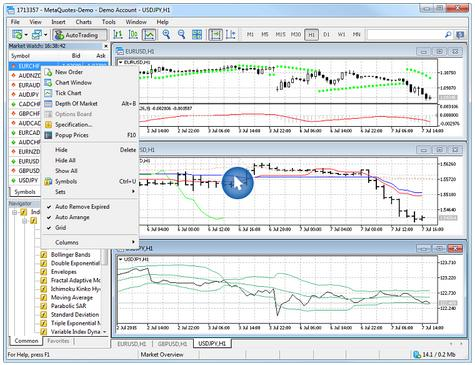
\includegraphics[width=0.85\textwidth]{fig01-interface-metatrader.png}
\fonte{\citeonline{metaquotes2024}.}
\end{figure}

A plataforma MetaTrader 5 (MT5), como se observa na imagem acima, oferece uma
interface personalizável que permite aos usuários organizarem múltiplas janelas de
acordo com suas preferências. A janela de Cotações exibe os preços em tempo real dos
instrumentos financeiros selecionados, e os Gráficos de Preços permitem visualizar a
evolução dos preços ao longo do tempo. O Navegador oferece acesso rápido a contas,
indicadores técnicos e scripts, facilitando a análise e o acompanhamento do mercado
\cite{metaquotes2024}.

\begin{figure}[htb]
\centering
\caption{Fluxograma do Funcionamento do EA}
\label{fig:fluxograma-ea}
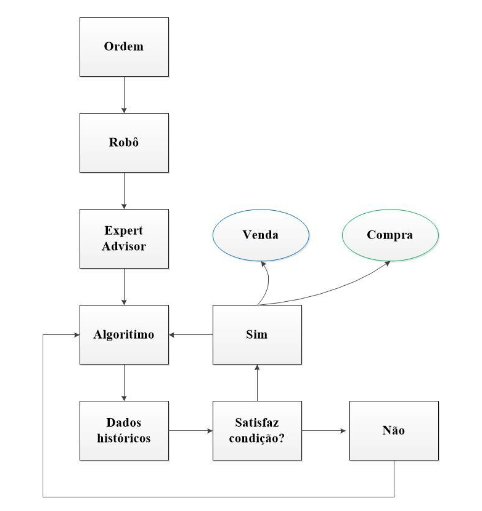
\includegraphics[width=0.55\textwidth]{fig02-fluxograma-ea.png}
\fonte{\citeonline{almeida2016}.}
\end{figure}

% TODO: citação (FLÁVIO, 2023) removida das duas frases abaixo — não há
% entrada correspondente em referencias.bib e a fonte não foi localizada.
% Confirmar a referência real e reinserir com \citeonline, ou manter sem
% citação caso a afirmação seja considerada conhecimento geral da área.
Um dos recursos mais poderosos do MT5 são os \textit{Expert Advisor}s (EAs), também conhecidos
como robôs de negociação. EAs são programas que automatizam o processo
de negociação, permitindo que os usuários executem estratégias complexas sem a
necessidade de intervenção manual. Esses robôs abrem, modificam e
fecham ordens automaticamente, com base em algoritmos predefinidos, e podem ser
criados tanto manualmente, para maior customização, quanto automaticamente, por meio
do MQL5 \cite{almeida2016}.

A análise técnica é um componente fundamental do MT5, com um conjunto abrangente de
ferramentas para a identificação de padrões e sinais de mercado. A plataforma oferece
uma variedade de indicadores técnicos integrados, abrangendo todas as principais
categorias, bem como objetos gráficos e ferramentas de desenho para uma análise
visual detalhada dos gráficos. A capacidade de analisar dados em múltiplos períodos,
desde M1 (1 minuto) até MN1 (1 mês), permite capturar padrões que podem não ser
evidentes em uma única escala temporal, resultando em algoritmos de previsão mais
robustos \cite{metaquotes2024}.

A negociação algorítmica é um dos pilares do MT5, devido à linguagem MQL5, que
permite criar EAs para a análise automatizada de dados de mercado, a geração de sinais
de negociação e a execução de ordens. O MetaEditor oferece um ambiente de
desenvolvimento completo, com recursos como destaque de sintaxe, compilador integrado
e depurador. O Testador de Estratégias possibilita a validação e otimização de
algoritmos utilizando dados históricos, com opções para testar em diferentes períodos
para simulação precisa e analisar estatísticas de desempenho detalhadas
\cite{metaquotes2024}.

A integração com Python, através de uma API dedicada, amplia as capacidades do MT5,
permitindo a utilização de bibliotecas de aprendizado de máquina e a criação de
modelos preditivos sofisticados. Essa integração possibilita a combinação das
funcionalidades nativas da plataforma com o poder analítico do ecossistema Python,
resultando em algoritmos de previsão mais precisos e adaptáveis. Adicionalmente, o
MT5 oferece suporte nativo para redes neurais em MQL5 e computação paralela com
OpenCL, fornecendo recursos avançados para o desenvolvimento de algoritmos
computacionalmente intensivos \cite{metaquotes2024}.

Em suma, o MetaTrader 5 se consolida como uma plataforma versátil e poderosa para o
desenvolvimento e a implementação de algoritmos de previsão de mercado. Sua
combinação de recursos nativos, integração com tecnologias externas e ecossistema
maduro o tornam uma escolha estratégica para pesquisadores, desenvolvedores e traders
que buscam criar sistemas preditivos sofisticados e eficientes para os mercados
financeiros.

\section{Indicadores}

Indicadores Técnicos são ferramentas fundamentais na análise estatística de mercados
financeiros, pois traduzem fórmulas matemáticas e gráficos de forma que auxiliam os
traders na tomada de decisões. Utilizando dados históricos de preço, volume, ou a
combinação de ambos, os indicadores buscam revelar padrões e tendências que, de outra
forma, seriam difíceis de discernir. Seu propósito principal é identificar potenciais
pontos de entrada e saída em negociações, sinalizar a força ou fraqueza de uma
tendência estabelecida, e demarcar zonas de suporte e resistência onde o preço tende
a encontrar dificuldades em romper \cite{fernandes2014}.

Embora baseados em cálculos estatísticos, os sinais gerados por indicadores técnicos
não devem ser interpretados como previsões infalíveis. Pelo contrário, eles funcionam
como alertas ou confirmações, que exigem uma análise cuidadosa e contextualizada por
parte do trader. A eficácia de um indicador pode variar significativamente entre
diferentes ativos e ao longo do tempo, exigindo um processo contínuo de adaptação e
ajuste de parâmetros \cite{fernandes2014}.

Em seguimento, alguns indicadores específicos serão explorados neste trabalho,
visando a identificação de tendências e a confirmação de sinais de negociação. A
escolha e a aplicação desses indicadores serão detalhadas nas seções subsequentes.

\subsection{Índice de Força Relativa}
De acordo com \citeonline{anderson1993}, o RSI é um dos mais conhecidos indicadores
de análise técnica e amplamente utilizado, não somente no mercado financeiro, mas
para medir a consolidação de uma tendência em diversas áreas. O índice é base para
diversos outros índices que necessitam de um norte para onde a tendência do ativo
aponta, sendo assim, uma ferramenta imprescindível para fomentar uma decisão
estratégica de entrada e saída de um ativo com maior segurança.

Diante do exposto, o Índice de Força Relativa tem como objetivo estudar posições
estratégicas no preço dos ativos para aproveitar-se de uma brecha de compra ou venda.

Sendo assim, as classificações de ativos por RSI são basicamente sobrevalorizados ou
supervalorizados; quando supervalorizado a melhor posição no ativo é de venda pois o
ativo vem esgotando sua força compradora devido ao preço inflado, em contrapartida, o
sobrevalorizado indica uma posição forte de compra pois, devido ao preço baixo, não
será recompensador para o investidor vender o ativo, criando-se uma resistência que
não propicia a vendas e sim compras.

\begin{figure}[htb]
\centering
\caption{Tendência de Alta com RSI}
\label{fig:rsi}
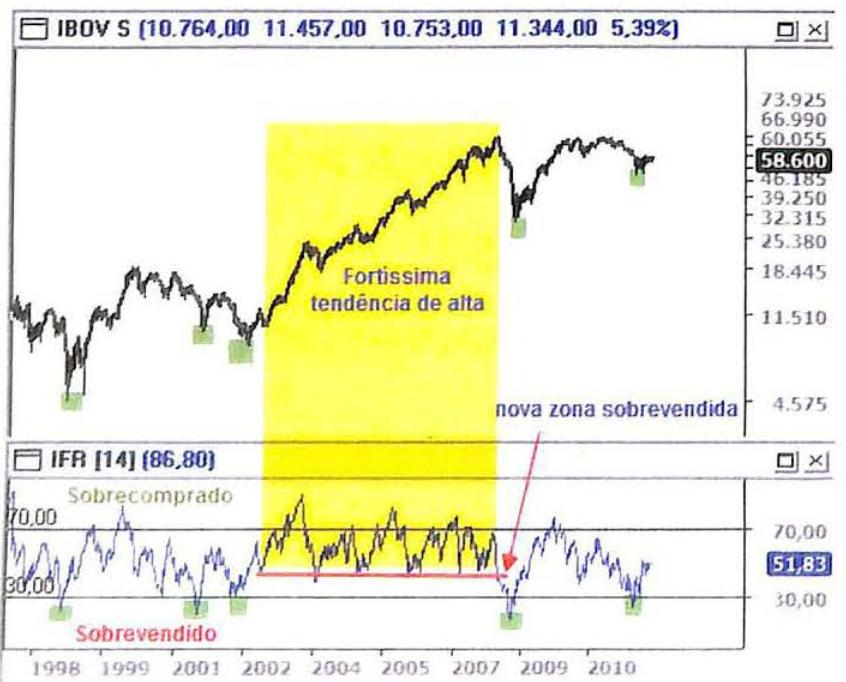
\includegraphics[width=0.8\textwidth]{fig03-tendencia-alta-rsi.png}
\fonte{\citeonline{fernandes2014}.}
\end{figure}

As margens de operação do RSI para compra e venda são frequentemente revisitadas; a
estrutura clássica diz que, abaixo de 30 pontos no índice, o ativo tende a subir pois
esgotou sua força vendedora, ao mesmo passo que, acima de 70 pontos no índice, o ativo
tende a cair pois esgotou sua força compradora. Levando em consideração todo o
contexto, o RSI não representa uma determinante que afirma o momento de compra ou
venda, o índice tem como objetivo ser uma ferramenta a mais para o consenso de
entradas e saídas em investimentos.

\subsection{Médias Móveis}
As Médias Móveis (MM) são um dos indicadores técnicos mais amplamente utilizados na
análise estatística de mercados financeiros, oferecendo uma maneira eficaz de suavizar
as flutuações de preço e identificar tendências predominantes. Ao calcular o preço
médio de um ativo durante um período específico, as Médias Móveis reduzem o ruído
gerado por movimentos de preço aleatórios, permitindo que os analistas visualizem a
direção geral do mercado com maior clareza, fornecendo pontos de referência válidos ao
longo do tempo, possibilitando a comparação entre níveis atuais e passados
\cite{fernandes2014}.

Existem diferentes tipos de Médias Móveis, sendo as mais comuns a Média Móvel Simples
(MMS) e a Média Móvel Exponencial (MME). A MMS atribui o mesmo peso a todos os preços
dentro do período, enquanto a MME pondera os preços mais recentes de forma mais
significativa, tornando-a mais sensível às mudanças de preço. A escolha entre MMS e
MME depende do objetivo da análise e da sensibilidade desejada. Períodos mais curtos
resultam em Médias Móveis mais sensíveis, que reagem rapidamente às mudanças de preço,
mas também geram mais sinais falsos. Períodos mais longos, por outro lado, resultam em
Médias Móveis mais suaves, que filtram o ruído, mas podem atrasar a identificação de
novas tendências \cite{fernandes2014}.

\begin{figure}[htb]
\centering
\caption{Cruzamento de médias móveis}
\label{fig:cruzamento-mm}
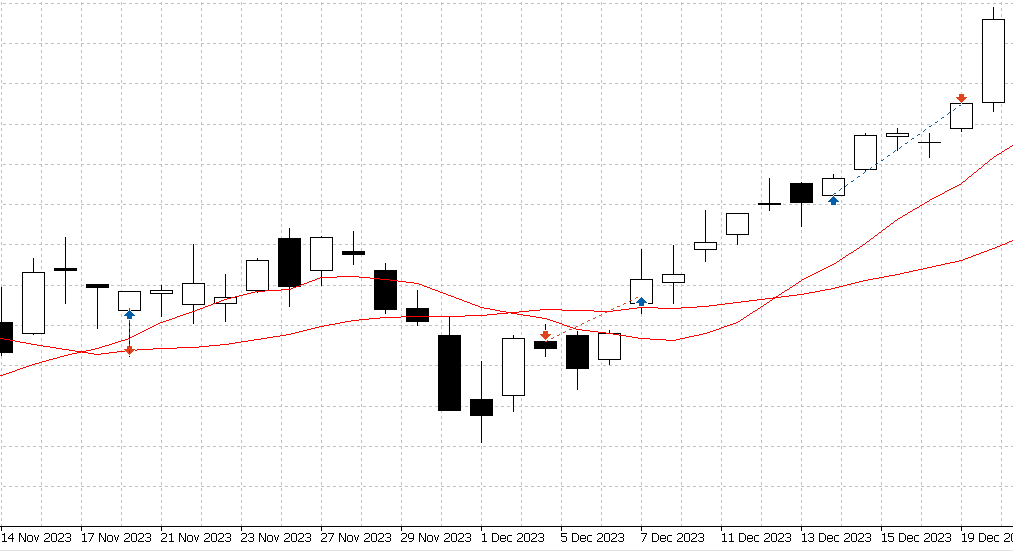
\includegraphics[width=0.95\textwidth]{fig04-cruzamento-medias.png}
\fonte{Elaboração própria com dados e interface do MetaTrader 5.}
\end{figure}

Uma aplicação comum das Médias Móveis, como é possível observar na imagem acima, é a
identificação de cruzamentos, interpretados como sinais de compra ou venda.
\citeonline{almeida2016}, em sua pesquisa, utilizou essa técnica com duas médias, uma
``rápida'' e outra ``lenta'', gerando sinais de negociação com base em seus
cruzamentos. Para um controle de risco mais refinado, implementou também StopLoss e
TakeProfit. Entretanto, \citeonline{almeida2016} alerta para as limitações de se usar
apenas essa técnica, especialmente em mercados com alta volatilidade, reforçando a
necessidade de ferramentas que confirmem o sinal para evitar falsos positivos.

\subsection{Médias Móveis Exponenciais}
As Médias Móveis Exponenciais (MME) constituem uma ferramenta amplamente conhecida na
análise técnica geral, destacando-se no mesmo sentido das médias móveis (MM), sendo
principalmente utilizada para suavizar alterações bruscas de curto prazo nos preços
dos ativos; além disso, atribui pesos mais acentuados para dados recentes. A diferença
entre os indicadores MM e MME é fundamentalmente velocidade: devido à fórmula adaptada
da MME, os resultados são mais velozes nas comparações utilizadas, contudo, o
processamento requisitado é maior. Por esse motivo, a MME é significativamente
utilizada em mercados de volatilidade pois é de suma importância identificar padrões
de reversões ou de continuidade num espaço de tempo consideravelmente curto para
tomadas de decisões.

Como já afirmado, a relevância da MME é ampla na área de análise técnica.
\citeonline{elder2002}, por exemplo, destaca o seu valor para análise de um mercado
atual, característica essa que é contrária em outros indicadores onde suas fórmulas não
consideram as datas dos dados extraídos. Segundo o autor, ``a média móvel exponencial
permite que o trader veja o mercado como ele é agora, e não como era semanas atrás''
\cite[p.~145]{elder2002}. Seguindo sua linha de pensamento, o cruzamento de médias
possui a capacidade de demonstrar sinais de entrada ou saída de forma eficaz.

Apesar de tantas vantagens, a MME também possui seus pontos de consideração. A
principal característica da MME é resultante da sua velocidade em extrair informações
que, em mercados de lateralização, gera sinais que podem ser interpretados como
falsos, levando a entradas e saídas em momentos desinteressantes. Uma forma de
diminuir esta influência é a complementação com outros indicadores, como por exemplo,
Índice de Força Relativa (IFR) ou Bandas de Bollinger; essa complementação cria dados
cruzados que confirmam uma incerteza ou uma compra, facilitando decisões.

\subsection{Bandas de Bollinger}
As Bandas de Bollinger (BB), um indicador técnico de volatilidade desenvolvido por
John Bollinger, oferecem uma perspectiva sobre a dinâmica dos preços em um mercado. As
BB são construídas a partir de uma Média Móvel Aritmética (MM20, por exemplo) aplicada
aos preços, traçando duas curvas que representam os limites superior e inferior da
volatilidade esperada para o ativo. Essas bandas são calculadas utilizando o desvio
padrão da média móvel, de modo que quanto maior a volatilidade do ativo, maior será a
distância entre as bandas \cite{fernandes2014}.

Ao contrário de uma interpretação simplista que considera a banda superior como uma
resistência e a banda inferior como um suporte, a teoria de Bollinger enfatiza a
importância de analisar o comportamento dos preços em relação aos seus limites de
volatilidade esperados. Se, em um movimento de alta, o preço atinge a banda superior,
isso indica força e sugere que o movimento deve prosseguir. Por outro lado, se o preço
não consegue alcançar a banda superior, isso pode ser um sinal de fraqueza. Da mesma
forma, a distância do preço em relação às bandas pode revelar informações importantes
sobre a intensidade dos movimentos de alta ou baixa \cite{fernandes2014}.

As Bandas de Bollinger (BB) permitem, adicionalmente, a avaliação da volatilidade do
mercado. Através do indicador BandWidth, derivado das BBs, é possível quantificar a
distância entre as bandas, oferecendo uma medida direta da volatilidade do ativo. A
ocorrência de períodos de baixa volatilidade, caracterizados pela aproximação das
bandas (squeeze), pode indicar um potencial transição para um período de alta
volatilidade (expansão), sinalizando oportunidades de negociação \cite{fernandes2014}.
Em sua pesquisa, Bertini (2024) empregou as Bandas de Bollinger para avaliar a
volatilidade de ativos, demonstrando a utilidade do indicador na seleção de ativos
para estratégias de negociação baseadas na identificação de períodos de variação
acentuada de preços.

\subsection{MACD}
O indicador MACD foi desenvolvido por Gerald Appel na década de 1970; sua proposta é
identificar mudanças no momentum do mercado \cite{appel2005}. Composto por duas
linhas, o MACD (Moving Average Convergence Divergence) representa a diferença entre
duas linhas de médias móveis exponenciais, respectivamente, 12 e 26 períodos; em
seguida, a linha que fornece sinal, média de 9 períodos, o indicador age no cruzamento
de todas as três médias.

Como destacado por \citeonline{elder2002}, o MACD é uma ferramenta interessante na
confirmação de tendências e em identificar pontos específicos de reversão. Geralmente
é utilizado em mercados com tendência mais previsível, mas por derivar da MME, pode
gerar falsos sinais em mercados de lateralidade. Por fim, outra característica
interessante é a capacidade de observar diferenças dos resultados MACD e da
movimentação nos preços, é outra aplicação interessante para a criação de Appel.

\section{Modelos Estatísticos}

Os modelos estatísticos representam uma abordagem fundamental na análise de dados,
especialmente em contextos em que se busca compreender padrões, relações e tendências.
Eles oferecem fórmulas estruturadas para interpretar informações históricas e, em
muitos casos, para projetar comportamentos futuros. Ao aplicar princípios matemáticos
e probabilísticos, esses modelos buscam simplificar a complexidade inerente aos
fenômenos observados, permitindo a extração de insights e a tomada de decisões baseada
em evidências quantitativas.

\subsection{ARIMA}
O modelo Autoregressive Integrated Moving Average (ARIMA) é um modelo estatístico
utilizado para análise de séries temporais. O ARIMA permite modelar dados que exibem
tendências e flutuações ao longo do tempo, sendo amplamente aplicado em áreas
financeiras para prever valores futuros com base em dados passados.

A estrutura do ARIMA é composta por três elementos: o componente Autoregressivo (AR),
que modela a influência dos valores passados da série no valor presente; a Média Móvel
(MA), que suaviza os ruídos e flutuações aleatórias presentes nos dados; e o Integrado
(I), responsável por tornar a série estacionária. Uma série estacionária apresenta
propriedades estatísticas constantes ao longo do tempo, ou seja, sua média e variância
não se alteram significativamente. Cada um desses componentes é definido por um
parâmetro: o parâmetro $p$ representa a ordem da autocorrelação, o parâmetro $q$ define
a ordem da média móvel, e o parâmetro $d$ determina o grau de diferenciação
\cite{xing2024}.

\begin{figure}[htb]
\centering
\caption{Fluxo ARIMA}
\label{fig:fluxo-arima}
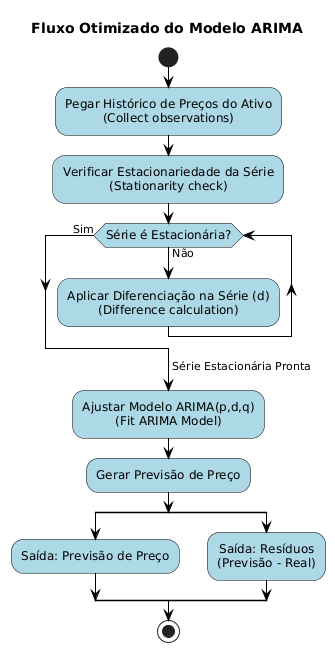
\includegraphics[width=0.4\textwidth]{fig05-fluxo-arima.png}
\fonte{Autoria própria.}
\end{figure}

Como é possível observar na figura acima, o processo de aplicação do modelo ARIMA
inicia-se com a coleta do histórico de preços do ativo. Em seguida, verifica-se a
estacionariedade da série; se não estiver estável, aplica-se a diferenciação
repetidamente até que a estabilidade seja alcançada. Com a série pronta, o modelo
ARIMA é ajustado, definindo-se suas ordens $p$, $d$ e $q$. Por fim, o modelo treinado
gera as previsões de preço e os resíduos, que representam os erros da previsão e são
importantes para análises futuras.

A verificação da estacionariedade e o subsequente ajuste dos parâmetros $p$, $d$ e $q$
são metodologicamente embasados em testes e critérios estatísticos. A etapa de
verificar a estacionariedade da série é formalmente conduzida por meio do teste de
Dickey-Fuller Aumentado (ADF). Este teste avalia a hipótese nula de que a série
temporal possui uma raiz unitária, sendo o p-valor resultante um indicador crucial: um
p-valor elevado, como o de 0,998773 encontrado inicialmente por
\citeonline{xing2024} para os dados da NVIDIA, impede a rejeição da hipótese nula,
confirmando a não estacionariedade. Já a aplicação da diferenciação repetidamente até
que a estabilidade seja alcançada é, portanto, guiada pelos resultados sequenciais do
teste ADF. No referido estudo, após a primeira diferenciação, um p-valor próximo de
zero indicou que a estacionariedade foi atingida, definindo assim $d=1$.

Subsequentemente, para o ajuste do modelo ARIMA, um passo crucial é a definição de
suas ordens $p$ (autorregressiva) e $q$ (médias móveis). Dada a multiplicidade de
combinações possíveis para estes parâmetros, como o intervalo de 0 a 4 testado por
\citeonline{xing2024}, torna-se necessário um critério objetivo para a seleção do
modelo mais apropriado. O \textit{Critério de Informação de Akaike} (\textit{AIC}) desempenha
precisamente este papel, sendo uma métrica estatística consolidada para avaliar a
qualidade relativa de diferentes modelos. O AIC permite selecionar a configuração que
oferece o melhor compromisso entre a fidelidade do modelo aos dados históricos
(qualidade do ajuste) e sua complexidade (parcimônia), penalizando modelos com excesso
de parâmetros que poderiam levar a overfitting. Assim, a configuração ARIMA que
resulta no menor valor de AIC é a escolhida, pois representa a estrutura mais eficiente
e generalizável, antes que o modelo treinado seja utilizado para gerar as previsões e
os resíduos \cite{xing2024}.

Uma outra variação do modelo ARIMA é o Seasonal Autoregressive Integrated Moving
Average, ou SARIMA, ideal para dados que exibem padrões sazonais. Ao contrário de
séries aleatórias, dados com sazonalidade apresentam comportamentos previsíveis que se
repetem em intervalos regulares, como vendas que aumentam no Natal ou no verão. O
SARIMA, além dos componentes AR, MA e I, incorpora componentes sazonais para capturar
esses padrões recorrentes, tornando-se uma ferramenta mais dimensionada para modelar
fenômenos com sazonalidade intrínseca \cite{araya2024}.

Apesar de sua utilidade, ambos os modelos apresentam limitações importantes. Sua
eficácia é maior na captura de relações lineares, o que dificulta lidar com padrões não
lineares complexos. Além disso, a escolha dos parâmetros ideais é um desafio, exigindo
análise criteriosa e experimentação. Em cenários complexos e não lineares, modelos de
aprendizado de máquina podem ser mais adequados \cite{araya2024,xing2024}.

\subsection{GARCH}
O modelo Generalized Autoregressive Conditional Heteroskedasticity (GARCH) é uma
ferramenta estatística para a análise de séries temporais financeiras, com foco na
modelagem da volatilidade. A volatilidade, como apontado por \citeonline{araya2024},
reflete o grau de variação dos preços de um ativo financeiro ao longo do tempo e é
fundamental para a gestão de riscos e a precificação de derivativos.

O objetivo principal do modelo GARCH é capturar a dependência temporal da
volatilidade, permitindo que ela varie dinamicamente em resposta às condições do
mercado. O modelo padrão, denominado SGARCH (Standard GARCH), considera que a
volatilidade atual é influenciada tanto pelos choques passados quanto pela própria
volatilidade passada, em um processo de retroalimentação como mostrado na imagem
abaixo \cite{araya2024}.

\begin{figure}[htb]
\centering
\caption{Fluxo GARCH}
\label{fig:fluxo-garch}
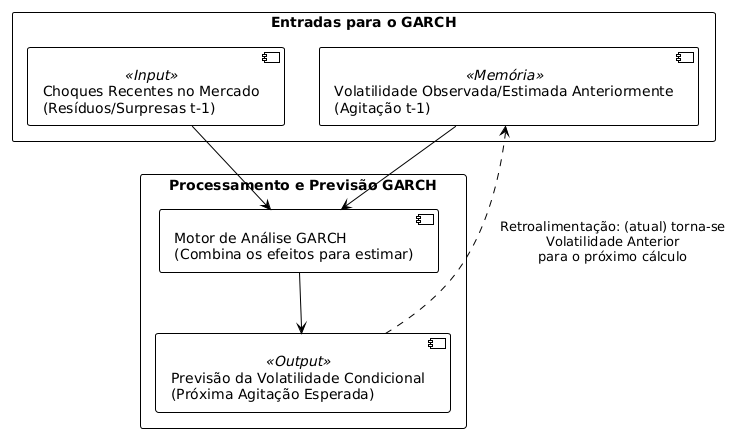
\includegraphics[width=0.7\textwidth]{fig06-fluxo-garch.png}
\fonte{Autoria própria.}
\end{figure}

No entanto, o modelo SGARCH assume que a resposta da volatilidade aos choques é
simétrica, ou seja, choques positivos e negativos de igual magnitude têm o mesmo
impacto na volatilidade. Essa premissa nem sempre se verifica nos mercados
financeiros, onde choques negativos (más notícias) frequentemente têm um impacto maior
do que choques positivos (boas notícias). Para lidar com essa assimetria, foram
desenvolvidas variações do modelo GARCH, como o EGARCH (Exponential GARCH) e o TGARCH
(Threshold GARCH) \cite{araya2024}.

O modelo EGARCH, por exemplo, permite que a volatilidade responda de forma diferente a
choques positivos e negativos, capturando o chamado efeito alavancagem. Já o modelo
TGARCH utiliza variáveis binárias (dummy variables) para identificar diferentes regimes
de volatilidade, permitindo que o modelo se adapte a diferentes condições de mercado
\cite{araya2024}.

A escolha entre o modelo SGARCH, EGARCH e TGARCH depende das características específicas
dos dados e dos objetivos da análise. \citeonline{araya2024} destaca essa importância
de selecionar o modelo mais adequado com base em métricas estatísticas.

\subsection{Integração ARIMA-GARCH}

A integração dos modelos ARIMA e GARCH representa uma abordagem robusta para a análise
de séries temporais financeiras, permitindo capturar tanto a tendência condicional
quanto a volatilidade condicional de um ativo. Conforme demonstrado por \citeonline{araya2024},
quando ARIMA e GARCH são combinados, os resíduos gerados pelo modelo ARIMA (que
representam os erros da previsão da média condicional) servem como série de entrada
para o modelo GARCH, que modela a variância condicional desses resíduos.


Essa integração é teoricamente fundamentada no trabalho seminal de \citeonline{bollerslev1986},
que estendeu os modelos de heteroscedasticidade condicional autorregressiva (\textit{ARCH})
inicialmente propostos por \citeonline{engle1982}. O modelo GARCH possibilita capturar
a dinâmica da volatilidade, que é crítica para a gestão de risco em mercados voláteis,
como no caso da ação PETR4, que apresenta elevadas flutuações de preço.


Na prática, a integração ARIMA-GARCH pode ser implementada por meio de três abordagens
estratégicas complementares. A primeira é o \textbf{Filtro de Volatilidade}, que restringe
operações a períodos em que a volatilidade prevista pelo GARCH permanece abaixo de um
limiar definido, reduzindo exposição a mercados instáveis. A segunda é a \textbf{Volatility Targeting}, que ajusta o tamanho da posição inversamente à volatilidade prevista,
diminuindo o risco relativo quando a incerteza aumenta. A terceira é o \textbf{Intervalo de Confiança}, que utiliza a volatilidade do GARCH para estabelecer limites superior
e inferior ao redor das previsões do ARIMA, criando uma zona de confiança para a entrada
e saída de operações.


Para aplicações em negociação de ativos voláteis, o \textbf{Filtro de Volatilidade}
emerge como a abordagem mais prudente, já que permite ao sistema evitar períodos de
heterocedasticidade elevada, alinhando-se ao objetivo de investimento seguro em ativos
com elevada variabilidade de preço. Essa estratégia garante que as operações ocorram
predominantemente em condições de mercado mais estáveis, reduzindo perdas relacionadas a
movimentos abruptos de preço.

\section{Trabalhos Relacionados}

Nesta seção são apresentados estudos e pesquisas relacionados ao tema deste trabalho. O
levantamento realizado foi orientado pela busca de pesquisas científicas e tecnológicas
que têm em seus objetivos o desenvolvimento, implementação e análise de ferramentas e
tecnologias para a previsão de séries temporais financeiras, análise de volatilidade e
desenvolvimento de estratégias de negociação algorítmica, com ênfase na aplicação de
modelos estatísticos e de aprendizado de máquina no mercado de ativos. A ferramenta que
serviu de referência para isso foi o Google Acadêmico e Publish or Perish 8, por meio
do qual se buscou mapear as pesquisas dessa natureza circunscritas nos últimos anos.

O estudo de \citeonline{almeida2016} figura como um precursor direto e ponto de partida
conceitual para o presente trabalho. Almeida investigou a aplicação de métodos
matemáticos e estatísticos no desenvolvimento de um robô de negociação, utilizando a
plataforma MetaTrader 5 e a linguagem MQL5, com foco específico no ativo PETR4. Sua
abordagem centrou-se na estratégia de cruzamento de médias móveis e na análise de
séries temporais com dados históricos, validando o robô através de backtests em
diferentes cenários, incluindo períodos de crise, e com o objetivo de alcançar um
retorno superior à taxa SELIC. O robô demonstrou viabilidade, apresentando
lucratividade em ativos de proteção e superando a SELIC com PETR4 fora de cenários de
crise, além de sugerir a exploração futura de modelos como o GARCH. A pesquisa de
Almeida é de fundamental importância para este TG, pois não apenas validou a utilização
do MetaTrader 5 e MQL5 para a análise algorítmica de PETR4, mas também serviu como base
para a ``revisitação e aplicação contemporânea'' que propomos, conforme mencionado na
justificativa deste projeto. Sua recomendação para explorar modelos mais robustos, como
o GARCH, alinhou-se com a intenção inicial deste trabalho de integrar também redes LSTM.
Embora esse componente tenha sido posteriormente excluído do escopo por limitações de
tempo e de ambiente de desenvolvimento (ver Capítulo 2, seção Obstáculos Encontrados), a
abordagem ARIMA-GARCH efetivamente implementada permitiu construir sobre os achados
iniciais de Almeida, buscando maior capacidade preditiva e adaptabilidade às atuais e
complexas condições do mercado brasileiro.

\citeonline{batista2024} desenvolveu um robô de investimento (\textit{Expert Advisor}) para
automatizar operações na bolsa de valores brasileira (B3), utilizando uma combinação
dos indicadores técnicos Média Móvel Exponencial, Convergência-Divergência de Médias
Móveis e Índice de Força Relativa visando lucros automatizados a médio e longo prazo.
Para isso, empregou a plataforma MetaTrader 5 e a linguagem MQL5, implementando uma
estratégia que integrava os sinais dos três indicadores para decisões de compra e
venda. A validação ocorreu por meio de backtests com dados históricos do ativo BBAS3F
de 2023, comparando o desempenho dos indicadores isoladamente, em pares e em conjunto.
Os resultados mostraram que a combinação dos três indicadores superou as abordagens com
menos indicadores, demonstrando a eficiência e consistência do EA nos testes e
indicando potencial para lucros automatizados.

Em 2022, \citeonline{silva2022} investigaram a previsão de tendências de preços de ações
da Petrobras (PETR4) no mercado brasileiro, com foco em operações intraday de 15
minutos, utilizando técnicas de inteligência artificial. Para isso, empregaram um
extrator de variáveis baseado em \textit{eXtreme Gradient Boosting} (\textit{XGBoost}) para selecionar os
indicadores técnicos mais relevantes dentre mais de 100 disponíveis, visando reduzir
ruído na amostra. Em seguida, uma rede neural \textit{Long Short-Term Memory} (\textit{LSTM}) foi aplicada
para prever a tendência de alta ou baixa dos preços no período de 2014 a 2020. Os
resultados alcançaram uma acurácia de 56\%, superando estudos anteriores, com melhor
desempenho na previsão de quedas (57\%) em comparação com altas (51\%), e destacando a
eficácia da combinação de \textit{XGBoost} para seleção de \textit{features} e \textit{LSTM} para previsão no
contexto do mercado financeiro brasileiro.

Em 2024, \citeonline{xing2024} realizaram uma análise comparativa de quatro modelos de
previsão -- ARIMA, \textit{Multilayer Perceptron} (\textit{MLP}), \textit{Long Short-Term Memory} (\textit{LSTM}) e um
modelo híbrido ARIMA-GARCH -- para prever o preço de fechamento ajustado do dia
seguinte das ações da NVIDIA. Utilizando dados diários da \textit{API} do \textit{Yahoo Finance} de abril
de 2019 a abril de 2024, o estudo dividiu o \textit{dataset} em 90\% para treino e 10\% para
teste. Os modelos \textit{LSTM} e \textit{MLP} foram configurados com janelas deslizantes, enquanto os
modelos ARIMA e ARIMA-GARCH utilizaram janelas expansivas e rolantes, com parâmetros
otimizados para o menor \textit{AIC}. Os resultados, avaliados por \textit{MAE}, \textit{RMSE} e \textit{R}-quadrado,
indicaram que o modelo ARIMA-GARCH apresentou o menor \textit{RMSE}, sugerindo melhor precisão na
previsão de grandes erros e na explicação da variância. No entanto, o modelo ARIMA com
janela expansiva demonstrou desempenho superior em geral, superando os modelos \textit{LSTM} e
\textit{MLP}, possivelmente devido às características predominantemente lineares da série temporal
e à sensibilidade dos modelos de \textit{deep learning} à configuração e ao tamanho da amostra.

\citeonline{araya2024} propuseram um método híbrido GARCH e \textit{Deep Learning} para predição
de volatilidade de preços de ações, visando aumentar a acurácia das previsões ao
integrar diversos modelos. O estudo combinou quatro abordagens: \textit{SARIMA} (\textit{Seasonal
Autoregressive Integrated Moving Average}), modelos da família GARCH (\textit{Generalized
Autoregressive Conditional Heteroskedasticity}), \textit{CNN} (\textit{Convolutional Neural Network}) e
\textit{BiLSTM} (\textit{Bidirectional Long Short-Term Memory}). Inicialmente, os resíduos gerados pelo
modelo \textit{SARIMA} foram utilizados como entrada para o modelo GARCH. Em seguida, a
volatilidade estimada por essa combinação serviu como \textit{feature} de entrada para os
modelos híbridos \textit{CNN} e \textit{BiLSTM}. A \textit{performance} do novo modelo híbrido proposto
(\textit{SARIMA-GARCH-CNN-BiLSTM}) foi avaliada utilizando métricas como \textit{MAE} (\textit{Mean Absolute
Error}) e \textit{RMSE} (\textit{Root Mean Squared Error}), demonstrando uma redução média significativa
nesses erros (60,35\% e 60,61\%, respectivamente) em comparação com outros modelos
híbridos. Os resultados experimentais indicaram que o modelo proposto apresentou bom
desempenho e acurácia na predição da volatilidade de preços de ações, oferecendo
\textit{insights} valiosos para análise de dados financeiros e estratégias de gerenciamento de
risco.

\citeonline{tormin2024} realizou um estudo comparativo entre os modelos ARIMA e \textit{LSTM}
para prever os retornos do Bitcoin, investigando o impacto da integração de dados de
tendências de busca do Google (\textit{PyTrends}) na capacidade preditiva. Utilizando dados
diários de preços do Bitcoin e tendências de busca para o termo ``Bitcoin'' de janeiro
de 2018 a outubro de 2024, foram construídos três modelos: ARIMA, \textit{LSTM} tradicional e
\textit{LSTM} integrado com \textit{PyTrends}. O pré-processamento incluiu ajuste ao fuso horário \textit{UTC},
tratamento de valores ausentes (\textit{fillna}) e normalização (\textit{MinMaxScaler}), com divisão de
80\% dos dados para treino e 20\% para teste. A avaliação, baseada em \textit{RMSE}, \textit{MAE} e \textit{MAPE},
mostrou que o ARIMA, apesar de simples, apresentou maior estabilidade em \textit{RMSE} e \textit{MAE}. O
\textit{LSTM} tradicional obteve \textit{RMSE} levemente melhor que o ARIMA, mas com \textit{MAPE}
significativamente mais alto. A inclusão dos dados do \textit{Google Trends} no modelo \textit{LSTM}
integrado não resultou em melhora significativa, sugerindo a necessidade de ajustes
mais robustos ou a inclusão de outras variáveis para capturar a complexidade do mercado
de criptomoedas.

\begin{table}[htb]
\centering
\caption{Tabela Comparativa}
\label{tab:comparativa}
\fontsize{10}{12}\selectfont
\begin{tabular}{lccc}
\toprule
\textbf{Estudo} & \textbf{Indicadores} & \textbf{Modelo estatístico} & \textbf{Machine Learning} \\
\midrule
(PEREIRA, 2025)         & X & X & X \\
(ALMEIDA, 2016)         & X & X &   \\
(BATISTA, 2024)         & X &   &   \\
(ARAYA, 2024)           &   & X & X \\
(SILVA, 2022)           & X &   & X \\
(XING, 2024)            &   & X & X \\
(TORMIN, 2024)          & X & X & X \\
\bottomrule
\end{tabular}

\vspace{2pt}
{\fontsize{10}{12}\selectfont Comparação entre as pesquisas, evidenciando quais
componentes cada uma utilizou para formular o modelo que elas propuseram.}
\fonte{Autoria própria.}
\end{table}

\begin{table}[htb]
\centering
\caption{Tabela Comparativa (Detalhada)}
\label{tab:comparativa-det}
\fontsize{9}{11}\selectfont
\begin{tabular}{p{2.0cm}cccp{1.6cm}p{1.8cm}p{1.4cm}p{1.8cm}}
\toprule
\textbf{Autor} & \textbf{Ativo Principal} & \textbf{Fonte de Dados} & \textbf{Tempo Gráfico} & \textbf{Indicadores} & \textbf{Modelo(s) Estatístico(s)} & \textbf{Modelo(s) de ML} & \textbf{Métricas para ML} \\
\midrule
(PEREIRA, 2025) & PETR4 & MetaTrader 5 & D1 & RSI, MME, MACD, BB & ARIMA, GARCH & LSTM & MAE, RMSE, R Square \\
(ALMEIDA, 2016) & PETR4 & MetaTrader 5 & D1 & MA & ARIMA, Encontro de Médias Móveis & -- & -- \\
(BATISTA, 2024) & BBAS3F & MetaTrader 5 & M30 & RSI, MME, MACD, BB & -- & -- & -- \\
(SILVA, 2022) & PETR4 & -- & M15 & 113 indicadores & -- & LSTM + XGBoost & Acurácia, Precision, Recall, F1-Score, Support \\
(XING, 2024) & NVIDIA (NVDA) & -- & -- & -- & ARIMA, GARCH & LSTM, MLP & MAE, RMSE, R Square \\
(ARAYA, 2024) & Apple Inc. (AAPL) & Yahoo Finance & D1 & -- & SARIMA, GARCH & CNN, Bi-LSTM & MAE, RMSE \\
(TORMIN, 2024) & Bitcoin (BTC-USD) & Google Trends & -- & -- & ARIMA & LSTM & MAE, RMSE, MAPE \\
\bottomrule
\end{tabular}

\vspace{2pt}
{\fontsize{10}{12}\selectfont Comparação entre as pesquisas, evidenciando as
características de cada uma em diversos aspectos.}
\fonte{Autoria própria.}
\end{table}

% =====================================================================
%  CAPÍTULO II / 3 Metodologia
% =====================================================================
\setdiv{CAPÍTULO II}
\chapter{Metodologia}

A metodologia deste trabalho foi estruturada em etapas sequenciais, visando o
desenvolvimento, implementação e validação da ferramenta algorítmica proposta para a
negociação de ativos financeiros. O objetivo foi descrever os passos para construir e
testar a solução, desde a escolha do ambiente até a avaliação de seu desempenho.

\section{Natureza da Pesquisa}

Este trabalho, como mencionado na introdução, adota uma natureza de pesquisa
experimental. A pesquisa experimental, no contexto de desenvolvimento de sistemas e
algoritmos, envolve a manipulação controlada de variáveis que, neste caso, foram os
parâmetros dos modelos, as combinações de indicadores técnicos, para observar e analisar
os efeitos resultantes em um ambiente controlado. Foram conduzidos experimentos para testar
diferentes configurações da ferramenta algorítmica, buscando identificar as abordagens
mais eficazes para a negociação do ativo financeiro selecionado \cite{wazlawick2014}.

\section{Padrões para Pesquisa Experimental}

Para a condução dos experimentos e o desenvolvimento da ferramenta algorítmica
proposta, foi utilizado um conjunto definido de padrões e ferramentas, cujas
funcionalidades e conceitos foram detalhados no capítulo anterior de Fundamentação
Teórica.

A plataforma MetaTrader 5 (MT5) foi empregada como o ambiente central para as fases
de desenvolvimento e teste. A linguagem de programação MQL5, nativa do MT5, foi
utilizada para a codificação dos \textit{Expert Advisors} (\textit{EAs}). Estes EAs são os algoritmos
que efetivamente incorporaram a lógica dos modelos de análise de tendência,
volatilidade e modelagem condicional para a execução automatizada de ordens
de negociação.

O testador de estratégias integrado ao MT5 foi uma ferramenta crucial, permitindo a
realização de backtests. Esses testes simularam o desempenho operacional das
estratégias desenvolvidas ao longo de períodos históricos, utilizando os dados de
cotações passadas para avaliar a viabilidade e a rentabilidade potencial.

Como fonte primária de dados, foi utilizado o banco de dados histórico de cotações
fornecido pela própria plataforma MetaTrader 5 com integração a corretoras
brasileiras. Inicialmente, a conta era integrada à corretora Rico, que permitia acessar
ações da B3. No entanto, durante o desenvolvimento, essa corretora cessou o fornecimento
de ativos para a plataforma MetaTrader 5, necessitando uma migração para a corretora
Clear, que mantém compatibilidade com a plataforma. Esta escolha metodológica simplificou
significativamente o processo de aquisição de dados, seu tratamento inicial e a
subsequente manipulação, uma vez que os dados se encontram em um formato padronizado
e são diretamente acessíveis via MQL5. Os dados extraídos e utilizados incluíram os
preços de abertura, máximo, mínimo e fechamento, bem como o volume de negociação para
cada período do timeframe definido para a análise, que foi diário (D1) para capturar
tendências mais longas.

O ativo referente às ações preferenciais da Petrobras (PETR4) foi o objeto de estudo
principal. Sua notória volatilidade histórica é um aspecto central para a aplicação
dos modelos subsequentes, em particular o modelo GARCH, que é projetado
especificamente para capturar e modelar a variância condicional em séries temporais
que exibem tais flutuações. A liquidez e a representatividade do PETR4 no Ibovespa
foram consideradas para assegurar a disponibilidade de dados robustos para esta
análise de volatilidade e para contextualizar os resultados no mercado acionário
nacional.

Para uma caracterização inicial e visualização dessa volatilidade inerente ao PETR4,
foram calculadas e analisadas as Bandas de Bollinger. Este indicador técnico, que
constrói um canal em torno de uma média móvel utilizando o desvio padrão dos preços,
foi aplicado à série histórica de preços do ativo. A observação da largura das bandas e
do comportamento do preço em relação a elas forneceu insights valiosos sobre os
diferentes regimes de variação dos preços (períodos de alta ou baixa volatilidade) e
contribuiu para a compreensão do ambiente de mercado no qual a ferramenta algorítmica
operaria.

\section{Obstáculos Encontrados}

Durante o desenvolvimento deste trabalho, foram enfrentados obstáculos significativos que impactaram o escopo e a execução da pesquisa.

\textbf{Perda do ambiente Windows e limitações no Linux:} O ambiente primário de desenvolvimento era uma máquina Windows, equipada com o MetaTrader 5 instalado nativamente. A perda desse equipamento obrigou a migração para um ambiente Linux (EndeavourOS), no qual o MetaTrader 5 não possui suporte oficial. A solução adotada foi executar a plataforma via Wine, o que, embora funcional, impõe limitações operacionais, como instabilidades ocasionais e restrições de compatibilidade com algumas APIs nativas da plataforma.

\textbf{Incompatibilidade da corretora Rico:} Durante a fase de coleta de dados e execução de backtests com ativos de ações, a corretora Rico cessou a disponibilização de ações em sua plataforma MetaTrader 5, inviabilizando o acesso ao ativo PETR4 através dessa conta. Foi necessário abrir uma nova conta na corretora Clear, que mantém compatibilidade com a plataforma, para dar continuidade à pesquisa. Esse processo causou atrasos e exigiu a reconfiguração do ambiente de testes.

Esses fatores combinados contribuíram para a redução do eescopo original (que previa a integração de modelos de \textit{Machine Learning}) concentrando o trabalho nos modelos ARIMA e GARCH.

\section{Experimento de Pesquisa}

O experimento de pesquisa iniciou-se com a implementação de abordagens para análise
de tendência utilizando Médias Móveis. Foram programados em MQL5 diferentes tipos de
médias móveis, como a Simples e a Exponencial. Estratégias baseadas em cruzamentos
dessas médias foram implementadas para gerar indicações preliminares sobre a direção
potencial do mercado, ou seja, sinais de compra ou venda. Estas estratégias também
serviram para verificar o desempenho de modelos baseados apenas em médias no mercado
mais recente.

Posteriormente, o experimento avançou para uma modelagem estatística mais sofisticada
da série temporal de preços, utilizando o modelo ARIMA. A determinação da ordem de
integração `d' do modelo ARIMA $(p, d, q)$ foi realizada através da aplicação
sequencial do teste de raiz unitária ADF sobre a série. Para a definição das ordens
autorregressiva `p' e de médias móveis `q', foi adotado um procedimento sistemático
de testar múltiplas combinações de 0 a 4. A seleção da especificação final foi
baseada no critério de informação \textit{Akaike Information Criterion} (\textit{AIC}).

Na sequência, os resíduos obtidos a partir do modelo ARIMA ajustado foram utilizados
como série de entrada para a modelagem da volatilidade condicional, por meio de um
modelo GARCH. Esta abordagem combinada, ARIMA-GARCH, visou capturar a dinâmica da
variância dos erros que não foi explicada pelo modelo de média condicional ARIMA.
Foram estimados modelos GARCH, com foco inicial e principal na especificação GARCH
(1,1), dada a sua prevalência e bom desempenho demonstrado na literatura para séries
temporais financeiras. O objetivo foi modelar e prever a volatilidade futura de curto
prazo dos resíduos, fornecendo uma medida do risco associado às previsões de preço do
ARIMA.

\section{Diagramas}

\begin{figure}[htb]
\centering
\caption{Modelo Completo}
\label{fig:modelo-completo}
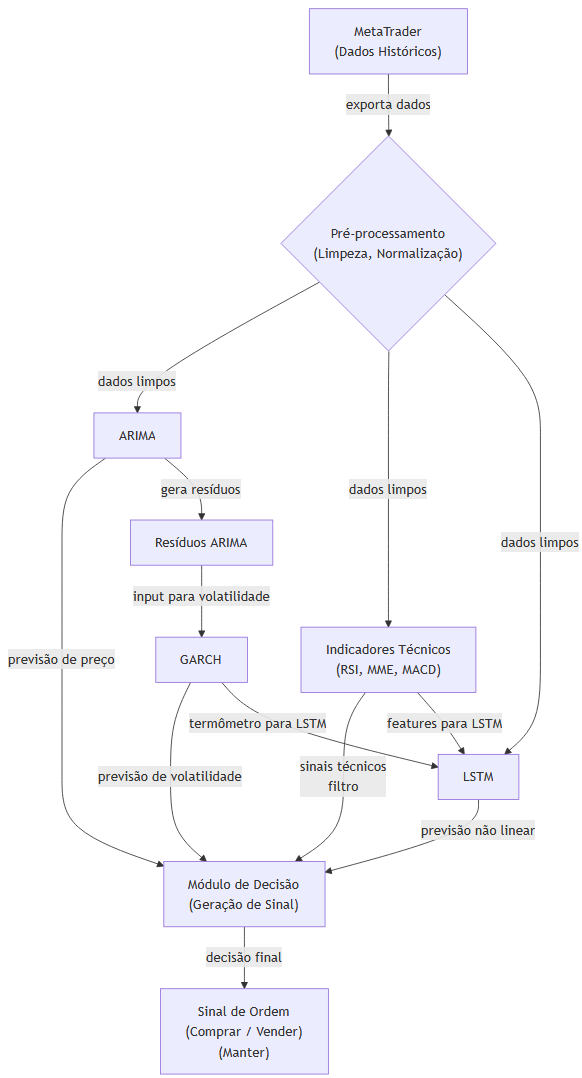
\includegraphics[width=0.45\textwidth]{fig08-modelo-completo.png}
\fonte{Autoria própria.}
\end{figure}

\section{Critérios para Avaliação}

Os testes das estratégias baseadas em Médias Móveis, cruzamento de Médias Móveis, e
dos modelos ARIMA e GARCH foram realizados integralmente na plataforma MetaTrader 5
por meio do ambiente de backtesting.

O desempenho dessas estratégias foi quantitativamente avaliado por meio de métricas
como a taxa de acerto das operações, o lucro ou prejuízo acumulado, o drawdown máximo
observado e o fator de lucro. Estas métricas foram fornecidas diretamente pela
plataforma. Adicionalmente, um critério importante para a validação interna dos modelos
estatísticos foi a qualidade do ajuste dos modelos ARIMA e GARCH. Esta qualidade foi
aferida utilizando o critério de informação Akaike (AIC) e pela verificação da
estacionariedade dos resíduos através do teste de raiz unitária de Dickey-Fuller
Aumentado (ADF).

\section{Resultados preliminares atingidos no PTG}

Como mencionado anteriormente, este projeto busca revisitar e expandir as investigações
de \citeonline{almeida2016}, que desenvolveu e testou um Expert Advisor (EA) baseado na
estratégia de cruzamento de Médias Móveis (MM) para o ativo PETR4 na plataforma
MetaTrader 5. O estudo original de \citeonline{almeida2016} observou que, embora sua
estratégia pudesse gerar lucros em determinados períodos de mercado mais estáveis, ela
enfrentava dificuldades e apresentava prejuízos durante crises financeiras,
evidenciando a sensibilidade do algoritmo simples às condições de mercado.

Para estabelecer um ponto de partida contemporâneo e avaliar o desempenho dessa
estratégia no cenário de mercado mais recente, foi necessário adaptar e reimplementar a
lógica central do EA proposto por \citeonline{almeida2016}.

O código original fornecido por ele, embora conceitualmente claro, demandou
atualizações para ser compatível com as versões mais recentes da linguagem MQL5 e da
plataforma MetaTrader 5. Adicionalmente, \citeonline{almeida2016} mencionou o uso de
bibliotecas externas para funcionalidades como gerenciamento de dinheiro e trailing
stops, as quais não foram disponibilizadas em seu trabalho. Desta forma, para a presente
análise preliminar, foi desenvolvido um EA em MQL5 utilizando a classe
CTrade\footnote{Biblioteca padrão do MQL5 para as operações de negociação.} padrão para
as operações de negociação e implementando a lógica de cruzamento de duas Médias Móveis
Simples (MMS).

A configuração do EA para este teste baseou-se nos seguintes parâmetros: Médias Móveis
Simples com período de 10 para a rápida e 20 para a lenta, aplicadas ao preço de
fechamento. A estratégia implementada inclui a reversão de posições, ou seja, ao ser
gerado um novo sinal, qualquer posição oposta existente é primeiramente fechada.

Os parâmetros de Stop Loss (SL) e Take Profit (TP) foram definidos por experimentação
inicial em 50 pontos e 100 pontos e depois nulos, respectivamente, uma vez que
\citeonline{almeida2016} não especificou os valores exatos utilizados em todos os seus
testes para PETR4. Reconhece-se que esta escolha de SL/TP pode divergir da utilizada
originalmente e constitui um ponto para otimizações e análises futuras.

As operações foram configuradas para serem executadas apenas na abertura de uma nova
barra no gráfico diário (D1), com a modelagem do backtest para \textit{Cada Tick} para maior
precisão na simulação dos preços de execução, alinhando-se com a abordagem de ``Every
tick'' mencionada por \citeonline{almeida2016}.

Visando uma comparação de desempenho sob condições financeiras similares às de um dos
cenários de \citeonline{almeida2016}, o backtest foi conduzido com um depósito inicial
de R\$ 50.000,00. O volume operacional foi definido como 1000 unidades do ativo PETR4
por negociação. A alavancagem utilizada na simulação foi de 1:100. O período de teste
compreendeu de 01 de janeiro de 2020 a 01 de maio de 2025.

Os principais resultados obtidos neste backtest para o ativo PETR4 são apresentados e
comparados qualitativamente com os achados de \citeonline{almeida2016} para PETR4 em
períodos de crise:

\begin{table}[htb]
\centering
\caption{Comparação modelo proposto x ALMEIDA (2016)}
\label{tab:comparacao-almeida}
\fontsize{10}{12}\selectfont
\begin{tabular}{lcccc}
\toprule
& \textbf{Pereira (2025)} & \textbf{Pereira (2025)} & \textbf{Almeida (2016)} & \textbf{Almeida (2016)} \\
& \textbf{1º teste} & \textbf{2º teste} & & \\
\midrule
\textbf{Período} & 2020-2025 (Crise) & 2020-2025 (Crise) & 2013-2016 & 2007-2011 (Crise) \\
\addlinespace
Volume por Operação & 1000 ações & 1000 ações & 1000 ações & 100 ações \\
Lucro Líquido Total & R\$ -9.230,00 & R\$ -2.530,00 & R\$ +10.430,00 & R\$ -2.542,00 \\
Retorno Percentual & -18,46\% & -5,06\% & +20,86\% & -5,08\% \\
Fator de Lucro & 0,64 & 0,93 & \textgreater{} 1,0 (lucro) & \textless{} 1,0 (prejuízo) \\
Total de Negociações & 64 & 58 & 38 & 52 \\
\bottomrule
\end{tabular}

\vspace{2pt}
\fonte{Elaboração própria com dados do MetaTrader 5 e pesquisa de \citeonline{almeida2016}.}
\end{table}

A análise destes resultados preliminares indica que, para o primeiro teste no período
recente de janeiro de 2020 a maio de 2025, a estratégia base de cruzamento de Médias
Móveis, operando com um volume de 1000 ações de PETR4, resultou em um prejuízo líquido
substancial de R\$ 9.230,00, representando uma perda de 18,46\% sobre o capital inicial.
O Fator de Lucro de 0,64 e a baixa taxa de acerto (apenas 25\% das 64 operações foram
lucrativas) confirmam a ineficácia da estratégia neste intervalo de tempo.

Em uma segunda rodada de testes preliminares para o período de janeiro de 2020 ao começo
de 2025 e mantendo o volume de 1000 ações de PETR4, foram zerados os parâmetros de Stop
Loss e Take Profit, resultando em um desempenho ligeiramente menos desfavorável. Neste
segundo cenário, o prejuízo líquido total foi de R\$ 2.530,00, correspondendo a uma
perda de 5,06\% sobre o capital inicial. Embora o Fator de Lucro tenha melhorado para
0,93 e o número total de negociações tenha sido reduzido para 58, a estratégia ainda não
demonstrou capacidade de gerar lucro. Este resultado, apesar de melhor que o anterior,
ainda se alinha com as dificuldades encontradas por \citeonline{almeida2016} em períodos
de crise e reforça a necessidade de abordagens mais robustas.

\begin{figure}[htb]
\centering
\caption{Desempenho do modelo proposto (2º teste)}
\label{fig:desempenho-2teste}
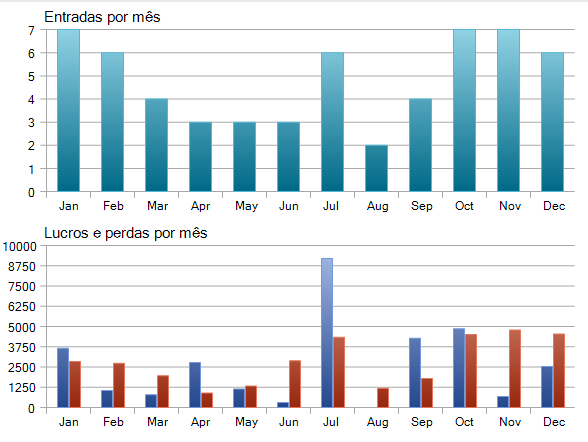
\includegraphics[width=0.8\textwidth]{fig09-desempenho-2teste.png}
\fonte{Elaboração própria com dados do MetaTrader 5.}
\end{figure}

\begin{figure}[htb]
\centering
\caption{Gráfico de dispersão da correlação de lucro (2º teste)}
\label{fig:dispersao-lucro}
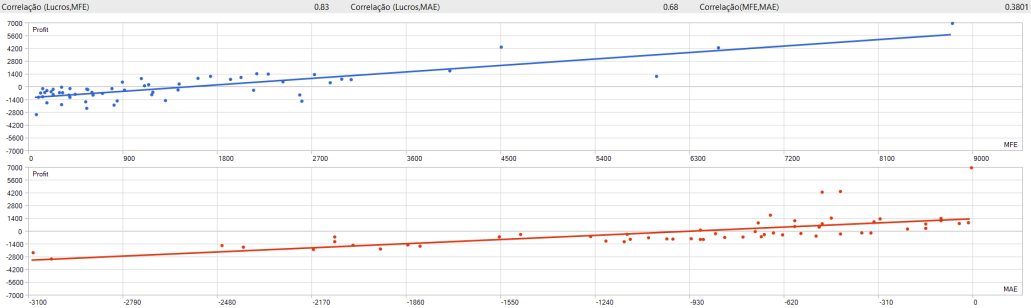
\includegraphics[width=0.9\textwidth]{fig10-dispersao-lucro.png}
\fonte{Elaboração própria com dados do MetaTrader 5.}
\end{figure}

Este desempenho contrasta significativamente com os resultados obtidos por
\citeonline{almeida2016} para o mesmo ativo e volume em um período anterior (2013-2016),
onde foi reportado um lucro considerável. Por outro lado, o resultado negativo atual se
assemelha, em natureza, aos prejuízos que Almeida também encontrou ao aplicar sua
estratégia em PETR4 durante períodos de crise financeira, como a de 2008.

O período de 2020-2025 foi caracterizado por uma volatilidade acentuada e por dinâmicas
de mercado complexas, influenciadas por eventos globais como a pandemia de COVID-19 e
suas repercussões econômicas. É plausível que tais condições tenham sido
particularmente desfavoráveis para uma estratégia de seguimento de tendência simples
como o cruzamento de médias. Adicionalmente, as necessárias adaptações do código
original de \citeonline{almeida2016} e a definição experimental dos parâmetros de Stop
Loss e Take Profit, na ausência dos valores exatos utilizados no estudo de referência,
são fatores que podem ter influenciado os resultados.

No entanto, a principal inferência destes testes preliminares é a clara demonstração de
que a estratégia de cruzamento de Médias Móveis, mesmo com parâmetros de risco básicos
e um volume operacional mais elevado, não se mostrou suficiente para gerar retornos
positivos de forma consistente no mercado recente de PETR4. Este achado é fundamental,
pois estabelece um baseline contemporâneo e valida de forma contundente a justificativa
central deste trabalho de graduação: a necessidade premente de investigar, desenvolver
e integrar modelos analíticos e preditivos mais sofisticados, como ARIMA para previsão
de tendência e GARCH para modelagem da volatilidade, com o objetivo de construir uma
ferramenta algorítmica mais robusta, adaptável e com maior potencial de eficácia para a
negociação de ativos voláteis no dinâmico cenário atual do mercado de ações brasileiro.

\section{Limitações e Trabalhos Futuros}

Os resultados finais de backtesting com os modelos ARIMA e GARCH ainda estão sendo consolidados e analisados. Os resultados preliminares obtidos com estratégias de Médias Móveis demonstraram a ineficácia de abordagens simplistas em cenários de mercado volátil, validando a necessidade de modelos mais sofisticados.

As limitações encontradas durante este trabalho incluem a restrição computacional e operacional do ambiente Linux via Wine, bem como as interrupções causadas pela mudança de corretora. Adicionalmente, o escopo reduzido — concentrado em ARIMA e GARCH — significa que componentes originalmente planejados, como a integração de Machine Learning (LSTM) para análises não lineares, não foram implementados neste ciclo.

Como perspectivas para trabalhos futuros, recomenda-se:

\begin{itemize}
  \item Implementação do modelo LSTM em um ambiente de desenvolvimento dedicado (Python com TensorFlow/Keras), seguido de integração ao MetaTrader 5 como componente complementar aos modelos ARIMA e GARCH;
  \item Incorporação de indicadores técnicos como filtro de confirmação (RSI, MACD) para validar sinais gerados pelos modelos estatísticos;
  \item Expansão da análise para outros ativos brasileiros de alta liquidez (ex., BBDC4, PETR3, VALE3) para validar a generalização da metodologia;
  \item Otimização de hiperparâmetros dos modelos ARIMA e GARCH através de algoritmos evolucionários (Genetic Algorithm, PSO);
  \item Implementação de técnicas robustas de gerenciamento de risco (trailing stops, position sizing dinâmico) para mitigação de drawdowns.
\end{itemize}


% ------------------------- Elementos pós-textuais --------------------
\postextual

\bibliography{referencias}

\begin{apendicesenv}
  \partapendices
  % No apêndice o cabeçalho deve exibir "APÊNDICE A – Título" no mesmo
  % tamanho dos demais títulos (13 pt); escopo local ao ambiente.
  \newcommand{\appchapfont}{\normalfont\bfseries\fontsize{14}{18}\selectfont}%
  \renewcommand{\printchaptername}{\appchapfont\MakeTextUppercase{\appendixname}\space}%
  \renewcommand{\printchapternum}{\chapnumberedtrue\appchapfont\thechapter}%
  \renewcommand{\afterchapternum}{\appchapfont\space\textendash\space}%
  \renewcommand{\printchaptertitle}[1]{\appchapfont #1}%
  % =====================================================================
%  APÊNDICE A — Código do Expert Advisor
% =====================================================================
\chapter{Algoritmo do Expert Advisor no MetaTrader 5}

Este apêndice apresenta o código fonte do \textit{Expert Advisor} baseado na estratégia de cruzamento de Médias Móveis, implementado conforme o trabalho de graduação de \citeonline{almeida2016} e as documentações oficiais do MetaTrader 5.

\lstinputlisting[style=mql5]{../MediasMoveis2/MediasMoveis2.mq5}

\end{apendicesenv}

\end{document}
